\documentclass[twoside]{book}

% Packages required by doxygen
\usepackage{fixltx2e}
\usepackage{calc}
\usepackage{doxygen}
\usepackage[export]{adjustbox} % also loads graphicx
\usepackage{graphicx}
\usepackage[utf8]{inputenc}
\usepackage{makeidx}
\usepackage{multicol}
\usepackage{multirow}
\PassOptionsToPackage{warn}{textcomp}
\usepackage{textcomp}
\usepackage[nointegrals]{wasysym}
\usepackage[table]{xcolor}

% Font selection
\usepackage[T1]{fontenc}
\usepackage[scaled=.90]{helvet}
\usepackage{courier}
\usepackage{amssymb}
\usepackage{sectsty}
\renewcommand{\familydefault}{\sfdefault}
\allsectionsfont{%
  \fontseries{bc}\selectfont%
  \color{darkgray}%
}
\renewcommand{\DoxyLabelFont}{%
  \fontseries{bc}\selectfont%
  \color{darkgray}%
}
\newcommand{\+}{\discretionary{\mbox{\scriptsize$\hookleftarrow$}}{}{}}

% Page & text layout
\usepackage{geometry}
\geometry{%
  a4paper,%
  top=2.5cm,%
  bottom=2.5cm,%
  left=2.5cm,%
  right=2.5cm%
}
\tolerance=750
\hfuzz=15pt
\hbadness=750
\setlength{\emergencystretch}{15pt}
\setlength{\parindent}{0cm}
\setlength{\parskip}{3ex plus 2ex minus 2ex}
\makeatletter
\renewcommand{\paragraph}{%
  \@startsection{paragraph}{4}{0ex}{-1.0ex}{1.0ex}{%
    \normalfont\normalsize\bfseries\SS@parafont%
  }%
}
\renewcommand{\subparagraph}{%
  \@startsection{subparagraph}{5}{0ex}{-1.0ex}{1.0ex}{%
    \normalfont\normalsize\bfseries\SS@subparafont%
  }%
}
\makeatother

% Headers & footers
\usepackage{fancyhdr}
\pagestyle{fancyplain}
\fancyhead[LE]{\fancyplain{}{\bfseries\thepage}}
\fancyhead[CE]{\fancyplain{}{}}
\fancyhead[RE]{\fancyplain{}{\bfseries\leftmark}}
\fancyhead[LO]{\fancyplain{}{\bfseries\rightmark}}
\fancyhead[CO]{\fancyplain{}{}}
\fancyhead[RO]{\fancyplain{}{\bfseries\thepage}}
\fancyfoot[LE]{\fancyplain{}{}}
\fancyfoot[CE]{\fancyplain{}{}}
\fancyfoot[RE]{\fancyplain{}{\bfseries\scriptsize Generated by Doxygen }}
\fancyfoot[LO]{\fancyplain{}{\bfseries\scriptsize Generated by Doxygen }}
\fancyfoot[CO]{\fancyplain{}{}}
\fancyfoot[RO]{\fancyplain{}{}}
\renewcommand{\footrulewidth}{0.4pt}
\renewcommand{\chaptermark}[1]{%
  \markboth{#1}{}%
}
\renewcommand{\sectionmark}[1]{%
  \markright{\thesection\ #1}%
}

% Indices & bibliography
\usepackage{natbib}
\usepackage[titles]{tocloft}
\setcounter{tocdepth}{3}
\setcounter{secnumdepth}{5}
\makeindex

% Hyperlinks (required, but should be loaded last)
\usepackage{ifpdf}
\ifpdf
  \usepackage[pdftex,pagebackref=true]{hyperref}
\else
  \usepackage[ps2pdf,pagebackref=true]{hyperref}
\fi
\hypersetup{%
  colorlinks=true,%
  linkcolor=blue,%
  citecolor=blue,%
  unicode%
}

% Custom commands
\newcommand{\clearemptydoublepage}{%
  \newpage{\pagestyle{empty}\cleardoublepage}%
}

\usepackage{caption}
\captionsetup{labelsep=space,justification=centering,font={bf},singlelinecheck=off,skip=4pt,position=top}

%===== C O N T E N T S =====

\begin{document}

% Titlepage & ToC
\hypersetup{pageanchor=false,
             bookmarksnumbered=true,
             pdfencoding=unicode
            }
\pagenumbering{roman}
\begin{titlepage}
\vspace*{7cm}
\begin{center}%
{\Large Final\+\_\+\+Project }\\
\vspace*{1cm}
{\large Generated by Doxygen 1.8.11}\\
\end{center}
\end{titlepage}
\clearemptydoublepage
\tableofcontents
\clearemptydoublepage
\pagenumbering{arabic}
\hypersetup{pageanchor=true}

%--- Begin generated contents ---
\chapter{Final Project}
\label{md_readme}
\hypertarget{md_readme}{}
\href{https://travis-ci.org/yhsueh/final_project}{\tt }

\subsection*{Project Descriptioin}

The project focus on a portion of the application of the ball collector robot. In a closed environment like cafe, the robot would detect the balls and move toward them based on the camera images. Once the robot gets to the object, the object would be removed. The final task is to remove all the objects present in the cafe.

\subsection*{Project Personnel}

The author of this R\+OS package is a second year master student enrolling at the University of Maryland at College Park. This pcakge is the final deliverable for the final project of the class software developement of robotics.

\subsection*{Disclaimer}

Copyright 2017 Yuyu\+Hsueh

Redistribution and use in source and binary forms, with or without modification, are permitted provided that the following conditions are met\+:


\begin{DoxyEnumerate}
\item Redistributions of source code must retain the above copyright notice, this list of conditions and the following disclaimer.
\item Redistributions in binary form must reproduce the above copyright notice, this list of conditions and the following disclaimer in the documentation and/or other materials provided with the distribution.
\item Neither the name of the copyright holder nor the names of its contributors may be used to endorse or promote products derived from this software without specific prior written permission.
\end{DoxyEnumerate}

T\+H\+IS S\+O\+F\+T\+W\+A\+RE IS P\+R\+O\+V\+I\+D\+ED BY T\+HE C\+O\+P\+Y\+R\+I\+G\+HT H\+O\+L\+D\+E\+RS A\+ND C\+O\+N\+T\+R\+I\+B\+U\+T\+O\+RS \char`\"{}\+A\+S I\+S\char`\"{} A\+ND A\+NY E\+X\+P\+R\+E\+SS OR I\+M\+P\+L\+I\+ED W\+A\+R\+R\+A\+N\+T\+I\+ES, I\+N\+C\+L\+U\+D\+I\+NG, B\+UT N\+OT L\+I\+M\+I\+T\+ED TO, T\+HE I\+M\+P\+L\+I\+ED W\+A\+R\+R\+A\+N\+T\+I\+ES OF M\+E\+R\+C\+H\+A\+N\+T\+A\+B\+I\+L\+I\+TY A\+ND F\+I\+T\+N\+E\+SS F\+OR A P\+A\+R\+T\+I\+C\+U\+L\+AR P\+U\+R\+P\+O\+SE A\+RE D\+I\+S\+C\+L\+A\+I\+M\+ED. IN NO E\+V\+E\+NT S\+H\+A\+LL T\+HE C\+O\+P\+Y\+R\+I\+G\+HT H\+O\+L\+D\+ER OR C\+O\+N\+T\+R\+I\+B\+U\+T\+O\+RS BE L\+I\+A\+B\+LE F\+OR A\+NY D\+I\+R\+E\+CT, I\+N\+D\+I\+R\+E\+CT, I\+N\+C\+I\+D\+E\+N\+T\+AL, S\+P\+E\+C\+I\+AL, E\+X\+E\+M\+P\+L\+A\+RY, OR C\+O\+N\+S\+E\+Q\+U\+E\+N\+T\+I\+AL D\+A\+M\+A\+G\+ES (I\+N\+C\+L\+U\+D\+I\+NG, B\+UT N\+OT L\+I\+M\+I\+T\+ED TO, P\+R\+O\+C\+U\+R\+E\+M\+E\+NT OF S\+U\+B\+S\+T\+I\+T\+U\+TE G\+O\+O\+DS OR S\+E\+R\+V\+I\+C\+ES; L\+O\+SS OF U\+SE, D\+A\+TA, OR P\+R\+O\+F\+I\+TS; OR B\+U\+S\+I\+N\+E\+SS I\+N\+T\+E\+R\+R\+U\+P\+T\+I\+ON) H\+O\+W\+E\+V\+ER C\+A\+U\+S\+ED A\+ND ON A\+NY T\+H\+E\+O\+RY OF L\+I\+A\+B\+I\+L\+I\+TY, W\+H\+E\+T\+H\+ER IN C\+O\+N\+T\+R\+A\+CT, S\+T\+R\+I\+CT L\+I\+A\+B\+I\+L\+I\+TY, OR T\+O\+RT (I\+N\+C\+L\+U\+D\+I\+NG N\+E\+G\+L\+I\+G\+E\+N\+CE OR O\+T\+H\+E\+R\+W\+I\+SE) A\+R\+I\+S\+I\+NG IN A\+NY W\+AY O\+UT OF T\+HE U\+SE OF T\+H\+IS S\+O\+F\+T\+W\+A\+RE, E\+V\+EN IF A\+D\+V\+I\+S\+ED OF T\+HE P\+O\+S\+S\+I\+B\+I\+L\+I\+TY OF S\+U\+CH D\+A\+M\+A\+GE.

\subsection*{Document Links\+:}

S\+IP Spreadsheet (Product Backlog and Iterations)\+: \href{https://docs.google.com/spreadsheets/d/12HwD9ipKP0mMze7esa8kOW532ijbNlVK7lirzBBcEvI/edit?usp=sharing}{\tt https\+://docs.\+google.\+com/spreadsheets/d/12\+Hw\+D9ip\+K\+P0m\+Mze7esa8k\+O\+W532ijb\+Nl\+V\+K7lirz\+B\+Bc\+Ev\+I/edit?usp=sharing}

Sprint Planning Notes and Review\+: \href{https://docs.google.com/document/d/1imp_Num2covjx0czFeErUQy3KCeT4MHiEl-_trNzzP8/edit?usp=sharing}{\tt https\+://docs.\+google.\+com/document/d/1imp\+\_\+\+Num2covjx0cz\+Fe\+Er\+U\+Qy3\+K\+Ce\+T4\+M\+Hi\+El-\/\+\_\+tr\+Nzz\+P8/edit?usp=sharing}

\subsection*{Build procedures\+:}


\begin{DoxyEnumerate}
\item Clone from github by inputting 
\begin{DoxyCode}
1 git clone -b FW3MultiThreading https://github.com/yhsueh/final\_project.git
\end{DoxyCode}

\item Make sure R\+O\+S\+\_\+\+P\+A\+C\+K\+A\+G\+E\+\_\+\+P\+A\+TH enviroment variable contain the workspace folder. This is done by sourcing the generated setup file under devel folder in the parent directory.
\item Input 
\begin{DoxyCode}
1 catkin\_make
\end{DoxyCode}
 to build the R\+OS package.
\end{DoxyEnumerate}

\subsection*{Procedures for running the turtlebot simulation\+:}


\begin{DoxyEnumerate}
\item Run roslaunch file to start gazebo, and two necessary nodes and a launch file. 
\begin{DoxyCode}
1 roslaunch final\_package turtle\_bot\_only\_world.launch
\end{DoxyCode}
 In a second terminal 
\begin{DoxyCode}
1 rosrun final\_package turtleCtrller
\end{DoxyCode}
 and 
\begin{DoxyCode}
1 rosrun final\_package base
\end{DoxyCode}
 N\+O\+TE\+: The nodes must be executed in this order. If the order is reversed, the program will result in unexpected condition.
\end{DoxyEnumerate}

\subsection*{Simple test}


\begin{DoxyEnumerate}
\item This test is just for verifying that the unit testing is configured correctly. 
\begin{DoxyCode}
1 cd <catkin\_ws>
2 catkin\_make run\_tests\_final\_package\_gtest\_base\_test
\end{DoxyCode}

\item Using rostest 
\begin{DoxyCode}
1 catkin\_make run\_tests\_final\_package
\end{DoxyCode}
 
\end{DoxyEnumerate}
\chapter{Class Index}
\section{Class List}
Here are the classes, structs, unions and interfaces with brief descriptions\+:\begin{DoxyCompactList}
\item\contentsline{section}{\hyperlink{classBase}{Base} }{\pageref{classBase}}{}
\item\contentsline{section}{\hyperlink{classCtrllerTest}{Ctrller\+Test} }{\pageref{classCtrllerTest}}{}
\item\contentsline{section}{\hyperlink{classImageProcess}{Image\+Process} }{\pageref{classImageProcess}}{}
\item\contentsline{section}{\hyperlink{classTurtleCtrl}{Turtle\+Ctrl} }{\pageref{classTurtleCtrl}}{}
\end{DoxyCompactList}

\chapter{File Index}
\section{File List}
Here is a list of all files with brief descriptions\+:\begin{DoxyCompactList}
\item\contentsline{section}{include/\hyperlink{Base_8hpp}{Base.\+hpp} \\*In this project, the nodes are being implemented as class objects. This is the header file for the base class }{\pageref{Base_8hpp}}{}
\item\contentsline{section}{include/\hyperlink{CtrllerTest_8hpp}{Ctrller\+Test.\+hpp} }{\pageref{CtrllerTest_8hpp}}{}
\item\contentsline{section}{include/\hyperlink{ImageProcess_8hpp}{Image\+Process.\+hpp} \\*This is a header file for \hyperlink{classImageProcess}{Image\+Process} class, processing the images gotten from the 3D sensor }{\pageref{ImageProcess_8hpp}}{}
\item\contentsline{section}{include/\hyperlink{TurtleCtrl_8hpp}{Turtle\+Ctrl.\+hpp} \\*The turtlectrller node has been implemented as a class. It has multiple services and publisher/subscribers in order to drive the turtlebot toward the ball objects }{\pageref{TurtleCtrl_8hpp}}{}
\item\contentsline{section}{src/\hyperlink{Base_8cpp}{Base.\+cpp} \\*\hyperlink{classBase}{Base} class implementation source file }{\pageref{Base_8cpp}}{}
\item\contentsline{section}{src/\hyperlink{base_8cpp}{base.\+cpp} \\*This is a source file for the base node of this project. The base node is responsible of getting and converting the images from the asus-\/xtion\+\_\+pro 3D sensor. Then, it passes these images into an \hyperlink{classImageProcess}{Image\+Process} object, which processes these images and search for the balls\textquotesingle{} centroids. Finally, the displacment between the center of the ball and the center of the image is published to the turtle\+Ctrller node in charge of the turtlebot actuator. In every iteration, the processed image would be displayed in an view window for users to see what the turtlebot sees. There are two services called to make sure all colors of balls are being collected. All the callbacks in this node are running at the rate of 5\+Hz }{\pageref{base_8cpp}}{}
\item\contentsline{section}{src/\hyperlink{ImageProcess_8cpp}{Image\+Process.\+cpp} \\*This node takes and analyze the range data. Subsequently, pass the the decision made based on the data to the turtle\+Ctrl node which manipulates the turtlebot }{\pageref{ImageProcess_8cpp}}{}
\item\contentsline{section}{src/\hyperlink{TurtleCtrl_8cpp}{Turtle\+Ctrl.\+cpp} \\*This is the implementation file for the \hyperlink{classTurtleCtrl}{Turtle\+Ctrl} class }{\pageref{TurtleCtrl_8cpp}}{}
\item\contentsline{section}{src/\hyperlink{turtleCtrl_8cpp}{turtle\+Ctrl.\+cpp} \\*This is the source code for the turtle\+Ctrller node, which has a simple PD controller that takes the displacement value as input. The output is published to the turtlebot actuator in terms of linear and angular velocities }{\pageref{turtleCtrl_8cpp}}{}
\item\contentsline{section}{test/\hyperlink{base__test_8cpp}{base\+\_\+test.\+cpp} \\*This is the testing file for the base node }{\pageref{base__test_8cpp}}{}
\item\contentsline{section}{test/\hyperlink{ctrller__test_8cpp}{ctrller\+\_\+test.\+cpp} \\*This is the testing file for ctrller node }{\pageref{ctrller__test_8cpp}}{}
\item\contentsline{section}{test/\hyperlink{CtrllerTest_8cpp}{Ctrller\+Test.\+cpp} \\*This is the C\+Trller\+Test class implementation file for the delete model callback used in ctrller\+\_\+test.  2017, Yuyu Hsueh }{\pageref{CtrllerTest_8cpp}}{}
\item\contentsline{section}{test/\hyperlink{imageProcess__test_8cpp}{image\+Process\+\_\+test.\+cpp} \\*This is the testing file for image\+Process class }{\pageref{imageProcess__test_8cpp}}{}
\end{DoxyCompactList}

\chapter{Class Documentation}
\hypertarget{classBase}{}\section{Base Class Reference}
\label{classBase}\index{Base@{Base}}


{\ttfamily \#include $<$Base.\+hpp$>$}

\subsection*{Public Member Functions}
\begin{DoxyCompactItemize}
\item 
\hyperlink{classBase_a5ffe0568374d8b9b4c4ec32953fd6453}{Base} ()
\begin{DoxyCompactList}\small\item\em Initialize publishers/subscribers/servers/clients and some constants. \end{DoxyCompactList}\item 
void \hyperlink{classBase_a07d8eb5e372ccab3c866c5abdce90d64}{image\+Callback} (const sensor\+\_\+msgs\+::\+Image\+Const\+Ptr \&msg)
\begin{DoxyCompactList}\small\item\em In this callback, the displacement of the centeroids of the balls and the image center is computed and passed to the turtlectrller node. A simple tracking check is added. If the displacment of an obect at one time is significantly smaller or larger than the displacment at last timestep, then the object detected is likely to be a different one. \end{DoxyCompactList}\item 
bool \hyperlink{classBase_a8b091924a7e8398ea11babdab370fd3f}{status\+Callback} (final\+\_\+package\+::\+Status\+Check\+::\+Request \&req, final\+\_\+package\+::\+Status\+Check\+::\+Response \&resp)
\begin{DoxyCompactList}\small\item\em This is the service callback from the turtle\+Ctrller node. \end{DoxyCompactList}\end{DoxyCompactItemize}
\subsection*{Public Attributes}
\begin{DoxyCompactItemize}
\item 
bool \hyperlink{classBase_a10b0afead866cc8cf2f5e2208a29d9f1}{complete\+Flag}
\item 
ros\+::\+Service\+Client \hyperlink{classBase_a874255744854a842b88ccab8674fca90}{color\+Change\+Cli\+\_\+}
\item 
int \hyperlink{classBase_af4c79a5d92200b5adf98634163333876}{color}
\end{DoxyCompactItemize}


\subsection{Detailed Description}
The base class initializes all the necessary publishers, subscribers, servers and clients. It also takes cares of the callbacks for subscribers and servers. It\textquotesingle{}s core function is to locate the ball objects and command the turtlebot to reach it. 

\subsection{Constructor \& Destructor Documentation}
\index{Base@{Base}!Base@{Base}}
\index{Base@{Base}!Base@{Base}}
\subsubsection[{\texorpdfstring{Base()}{Base()}}]{\setlength{\rightskip}{0pt plus 5cm}Base\+::\+Base (
\begin{DoxyParamCaption}
{}
\end{DoxyParamCaption}
)}\hypertarget{classBase_a5ffe0568374d8b9b4c4ec32953fd6453}{}\label{classBase_a5ffe0568374d8b9b4c4ec32953fd6453}


Initialize publishers/subscribers/servers/clients and some constants. 


\begin{DoxyParams}{Parameters}
{\em none} & \\
\hline
\end{DoxyParams}
\begin{DoxyReturn}{Returns}
none 
\end{DoxyReturn}


\subsection{Member Function Documentation}
\index{Base@{Base}!image\+Callback@{image\+Callback}}
\index{image\+Callback@{image\+Callback}!Base@{Base}}
\subsubsection[{\texorpdfstring{image\+Callback(const sensor\+\_\+msgs\+::\+Image\+Const\+Ptr \&msg)}{imageCallback(const sensor_msgs::ImageConstPtr &msg)}}]{\setlength{\rightskip}{0pt plus 5cm}void Base\+::image\+Callback (
\begin{DoxyParamCaption}
\item[{const sensor\+\_\+msgs\+::\+Image\+Const\+Ptr \&}]{msg}
\end{DoxyParamCaption}
)}\hypertarget{classBase_a07d8eb5e372ccab3c866c5abdce90d64}{}\label{classBase_a07d8eb5e372ccab3c866c5abdce90d64}


In this callback, the displacement of the centeroids of the balls and the image center is computed and passed to the turtlectrller node. A simple tracking check is added. If the displacment of an obect at one time is significantly smaller or larger than the displacment at last timestep, then the object detected is likely to be a different one. 

The camera images are obtained from the 3D sensor. These images are passed to an imageprocess object for further image analysis. At the end, the centroid of the detected circles are computed.


\begin{DoxyParams}{Parameters}
{\em sensor\+\_\+msg\+::\+Image\+Const\+Ptr\&} & msg \\
\hline
\end{DoxyParams}
\begin{DoxyReturn}{Returns}
none 
\end{DoxyReturn}
\index{Base@{Base}!status\+Callback@{status\+Callback}}
\index{status\+Callback@{status\+Callback}!Base@{Base}}
\subsubsection[{\texorpdfstring{status\+Callback(final\+\_\+package\+::\+Status\+Check\+::\+Request \&req, final\+\_\+package\+::\+Status\+Check\+::\+Response \&resp)}{statusCallback(final_package::StatusCheck::Request &req, final_package::StatusCheck::Response &resp)}}]{\setlength{\rightskip}{0pt plus 5cm}bool Base\+::status\+Callback (
\begin{DoxyParamCaption}
\item[{final\+\_\+package\+::\+Status\+Check\+::\+Request \&}]{req, }
\item[{final\+\_\+package\+::\+Status\+Check\+::\+Response \&}]{resp}
\end{DoxyParamCaption}
)}\hypertarget{classBase_a8b091924a7e8398ea11babdab370fd3f}{}\label{classBase_a8b091924a7e8398ea11babdab370fd3f}


This is the service callback from the turtle\+Ctrller node. 

This function is the service callback from the turtle\+Ctrller node. It recieves a request when a model in Gazebo is removed.


\begin{DoxyParams}{Parameters}
{\em Status\+Check} & service request and respond. \\
\hline
\end{DoxyParams}
\begin{DoxyReturn}{Returns}
true 
\end{DoxyReturn}


\subsection{Member Data Documentation}
\index{Base@{Base}!color@{color}}
\index{color@{color}!Base@{Base}}
\subsubsection[{\texorpdfstring{color}{color}}]{\setlength{\rightskip}{0pt plus 5cm}int Base\+::color}\hypertarget{classBase_af4c79a5d92200b5adf98634163333876}{}\label{classBase_af4c79a5d92200b5adf98634163333876}
1\+:Red, 2\+:Green, 3\+:Blue \index{Base@{Base}!color\+Change\+Cli\+\_\+@{color\+Change\+Cli\+\_\+}}
\index{color\+Change\+Cli\+\_\+@{color\+Change\+Cli\+\_\+}!Base@{Base}}
\subsubsection[{\texorpdfstring{color\+Change\+Cli\+\_\+}{colorChangeCli_}}]{\setlength{\rightskip}{0pt plus 5cm}ros\+::\+Service\+Client Base\+::color\+Change\+Cli\+\_\+}\hypertarget{classBase_a874255744854a842b88ccab8674fca90}{}\label{classBase_a874255744854a842b88ccab8674fca90}
Tells the turtlebot which color ball to collect \index{Base@{Base}!complete\+Flag@{complete\+Flag}}
\index{complete\+Flag@{complete\+Flag}!Base@{Base}}
\subsubsection[{\texorpdfstring{complete\+Flag}{completeFlag}}]{\setlength{\rightskip}{0pt plus 5cm}bool Base\+::complete\+Flag}\hypertarget{classBase_a10b0afead866cc8cf2f5e2208a29d9f1}{}\label{classBase_a10b0afead866cc8cf2f5e2208a29d9f1}


The documentation for this class was generated from the following files\+:\begin{DoxyCompactItemize}
\item 
include/\hyperlink{Base_8hpp}{Base.\+hpp}\item 
src/\hyperlink{Base_8cpp}{Base.\+cpp}\end{DoxyCompactItemize}

\hypertarget{classImageProcess}{}\section{Image\+Process Class Reference}
\label{classImageProcess}\index{Image\+Process@{Image\+Process}}


{\ttfamily \#include $<$Image\+Process.\+hpp$>$}

\subsection*{Public Member Functions}
\begin{DoxyCompactItemize}
\item 
\hyperlink{classImageProcess_a3dd8d2b73be1d21ccac33921defcf533}{Image\+Process} ()
\item 
void \hyperlink{classImageProcess_a4c08cfba39236fa09ec5f2d0e37452fb}{load\+Image} (const cv\+::\+Mat \&)
\item 
void \hyperlink{classImageProcess_a0a4d4d847095fa9632565ec68b746b4f}{detection} ()
\begin{DoxyCompactList}\small\item\em Based on the color chosen in the range from 1 to 3, the corresponding filter will be applied in H\+SV color space. If no color is specified, it would do nothing and await next callback. \end{DoxyCompactList}\item 
const cv\+::\+Mat \& \hyperlink{classImageProcess_abedcfaaa343e334b5bc09a45e69c92ba}{get\+Image} ()
\item 
int \hyperlink{classImageProcess_a98f98b789934e466c504977d3af3f031}{get\+Color} ()
\end{DoxyCompactItemize}
\subsection*{Public Attributes}
\begin{DoxyCompactItemize}
\item 
std\+::vector$<$ cv\+::\+Vec3f $>$ \hyperlink{classImageProcess_aafcbd180aa8e8dd937f736a43685a6bc}{circles}
\item 
bool \hyperlink{classImageProcess_a265b78fb51ab67a89743dd9c3f85e69b}{detect\+Flag}
\item 
int \hyperlink{classImageProcess_ab96f8c1ee03f6bbf8e60ffa496fdaa0d}{color}
\end{DoxyCompactItemize}


\subsection{Detailed Description}
The image\+Process class loads the image and detects the centroids of the detected circles. 

\subsection{Constructor \& Destructor Documentation}
\index{Image\+Process@{Image\+Process}!Image\+Process@{Image\+Process}}
\index{Image\+Process@{Image\+Process}!Image\+Process@{Image\+Process}}
\subsubsection[{\texorpdfstring{Image\+Process()}{ImageProcess()}}]{\setlength{\rightskip}{0pt plus 5cm}Image\+Process\+::\+Image\+Process (
\begin{DoxyParamCaption}
{}
\end{DoxyParamCaption}
)\hspace{0.3cm}{\ttfamily [inline]}}\hypertarget{classImageProcess_a3dd8d2b73be1d21ccac33921defcf533}{}\label{classImageProcess_a3dd8d2b73be1d21ccac33921defcf533}


\subsection{Member Function Documentation}
\index{Image\+Process@{Image\+Process}!detection@{detection}}
\index{detection@{detection}!Image\+Process@{Image\+Process}}
\subsubsection[{\texorpdfstring{detection()}{detection()}}]{\setlength{\rightskip}{0pt plus 5cm}void Image\+Process\+::detection (
\begin{DoxyParamCaption}
{}
\end{DoxyParamCaption}
)}\hypertarget{classImageProcess_a0a4d4d847095fa9632565ec68b746b4f}{}\label{classImageProcess_a0a4d4d847095fa9632565ec68b746b4f}


Based on the color chosen in the range from 1 to 3, the corresponding filter will be applied in H\+SV color space. If no color is specified, it would do nothing and await next callback. 


\begin{DoxyParams}{Parameters}
{\em none;} & \\
\hline
\end{DoxyParams}
\begin{DoxyReturn}{Returns}
none; 
\end{DoxyReturn}
\index{Image\+Process@{Image\+Process}!get\+Color@{get\+Color}}
\index{get\+Color@{get\+Color}!Image\+Process@{Image\+Process}}
\subsubsection[{\texorpdfstring{get\+Color()}{getColor()}}]{\setlength{\rightskip}{0pt plus 5cm}int Image\+Process\+::get\+Color (
\begin{DoxyParamCaption}
{}
\end{DoxyParamCaption}
)\hspace{0.3cm}{\ttfamily [inline]}}\hypertarget{classImageProcess_a98f98b789934e466c504977d3af3f031}{}\label{classImageProcess_a98f98b789934e466c504977d3af3f031}
\index{Image\+Process@{Image\+Process}!get\+Image@{get\+Image}}
\index{get\+Image@{get\+Image}!Image\+Process@{Image\+Process}}
\subsubsection[{\texorpdfstring{get\+Image()}{getImage()}}]{\setlength{\rightskip}{0pt plus 5cm}const cv\+::\+Mat\& Image\+Process\+::get\+Image (
\begin{DoxyParamCaption}
{}
\end{DoxyParamCaption}
)\hspace{0.3cm}{\ttfamily [inline]}}\hypertarget{classImageProcess_abedcfaaa343e334b5bc09a45e69c92ba}{}\label{classImageProcess_abedcfaaa343e334b5bc09a45e69c92ba}
\index{Image\+Process@{Image\+Process}!load\+Image@{load\+Image}}
\index{load\+Image@{load\+Image}!Image\+Process@{Image\+Process}}
\subsubsection[{\texorpdfstring{load\+Image(const cv\+::\+Mat \&)}{loadImage(const cv::Mat &)}}]{\setlength{\rightskip}{0pt plus 5cm}void Image\+Process\+::load\+Image (
\begin{DoxyParamCaption}
\item[{const cv\+::\+Mat \&}]{img}
\end{DoxyParamCaption}
)}\hypertarget{classImageProcess_a4c08cfba39236fa09ec5f2d0e37452fb}{}\label{classImageProcess_a4c08cfba39236fa09ec5f2d0e37452fb}


\subsection{Member Data Documentation}
\index{Image\+Process@{Image\+Process}!circles@{circles}}
\index{circles@{circles}!Image\+Process@{Image\+Process}}
\subsubsection[{\texorpdfstring{circles}{circles}}]{\setlength{\rightskip}{0pt plus 5cm}std\+::vector$<$cv\+::\+Vec3f$>$ Image\+Process\+::circles}\hypertarget{classImageProcess_aafcbd180aa8e8dd937f736a43685a6bc}{}\label{classImageProcess_aafcbd180aa8e8dd937f736a43685a6bc}
\index{Image\+Process@{Image\+Process}!color@{color}}
\index{color@{color}!Image\+Process@{Image\+Process}}
\subsubsection[{\texorpdfstring{color}{color}}]{\setlength{\rightskip}{0pt plus 5cm}int Image\+Process\+::color}\hypertarget{classImageProcess_ab96f8c1ee03f6bbf8e60ffa496fdaa0d}{}\label{classImageProcess_ab96f8c1ee03f6bbf8e60ffa496fdaa0d}
\index{Image\+Process@{Image\+Process}!detect\+Flag@{detect\+Flag}}
\index{detect\+Flag@{detect\+Flag}!Image\+Process@{Image\+Process}}
\subsubsection[{\texorpdfstring{detect\+Flag}{detectFlag}}]{\setlength{\rightskip}{0pt plus 5cm}bool Image\+Process\+::detect\+Flag}\hypertarget{classImageProcess_a265b78fb51ab67a89743dd9c3f85e69b}{}\label{classImageProcess_a265b78fb51ab67a89743dd9c3f85e69b}


The documentation for this class was generated from the following files\+:\begin{DoxyCompactItemize}
\item 
include/\hyperlink{ImageProcess_8hpp}{Image\+Process.\+hpp}\item 
src/\hyperlink{ImageProcess_8cpp}{Image\+Process.\+cpp}\end{DoxyCompactItemize}

\hypertarget{classTurtleCtrl}{}\section{Turtle\+Ctrl Class Reference}
\label{classTurtleCtrl}\index{Turtle\+Ctrl@{Turtle\+Ctrl}}


{\ttfamily \#include $<$Turtle\+Ctrl.\+hpp$>$}

\subsection*{Public Member Functions}
\begin{DoxyCompactItemize}
\item 
\hyperlink{classTurtleCtrl_ad74e99396945d2234307c91467baab2b}{Turtle\+Ctrl} ()
\item 
void \hyperlink{classTurtleCtrl_aa5c2960884f7c171bee34ac1f0d867c6}{disp\+Callback} (const std\+\_\+msgs\+::\+Int64 \&disp\+Msg)
\begin{DoxyCompactList}\small\item\em This callback controls the actuator of the turtlebot. When nothing is detected, the disp is passed in as 10000. \end{DoxyCompactList}\item 
void \hyperlink{classTurtleCtrl_ae68f9b9b0f40ae07d68332625ac75440}{range\+Callback} (const sensor\+\_\+msgs\+::\+Laser\+Scan\+::\+Const\+Ptr \&msg)
\item 
bool \hyperlink{classTurtleCtrl_aa803104f5e820d420927df598e48f924}{color\+Callback} (final\+\_\+package\+::\+Color\+Change\+::\+Request \&req, final\+\_\+package\+::\+Color\+Change\+::\+Response \&resp)
\begin{DoxyCompactList}\small\item\em This callback speicifies the color. \end{DoxyCompactList}\end{DoxyCompactItemize}
\subsection*{Public Attributes}
\begin{DoxyCompactItemize}
\item 
ros\+::\+Service\+Client \hyperlink{classTurtleCtrl_aa9a72ccbacd4c55c356ba0305ba14a4a}{status\+Check\+Cli\+\_\+}
\item 
bool \hyperlink{classTurtleCtrl_a0022c4d538eef753a0d49d4dfbdd4549}{terminate}
\end{DoxyCompactItemize}


\subsection{Constructor \& Destructor Documentation}
\index{Turtle\+Ctrl@{Turtle\+Ctrl}!Turtle\+Ctrl@{Turtle\+Ctrl}}
\index{Turtle\+Ctrl@{Turtle\+Ctrl}!Turtle\+Ctrl@{Turtle\+Ctrl}}
\subsubsection[{\texorpdfstring{Turtle\+Ctrl()}{TurtleCtrl()}}]{\setlength{\rightskip}{0pt plus 5cm}Turtle\+Ctrl\+::\+Turtle\+Ctrl (
\begin{DoxyParamCaption}
{}
\end{DoxyParamCaption}
)}\hypertarget{classTurtleCtrl_ad74e99396945d2234307c91467baab2b}{}\label{classTurtleCtrl_ad74e99396945d2234307c91467baab2b}
Constrcutor that initialize pubs/subs/servers/clients

The constructor for the turtlectrl node class. Kp and Kd gains are initialized here along with all other pubs/subs/servers/clients. The maixmum angular velocities are 0.\+15. 

\subsection{Member Function Documentation}
\index{Turtle\+Ctrl@{Turtle\+Ctrl}!color\+Callback@{color\+Callback}}
\index{color\+Callback@{color\+Callback}!Turtle\+Ctrl@{Turtle\+Ctrl}}
\subsubsection[{\texorpdfstring{color\+Callback(final\+\_\+package\+::\+Color\+Change\+::\+Request \&req, final\+\_\+package\+::\+Color\+Change\+::\+Response \&resp)}{colorCallback(final_package::ColorChange::Request &req, final_package::ColorChange::Response &resp)}}]{\setlength{\rightskip}{0pt plus 5cm}bool Turtle\+Ctrl\+::color\+Callback (
\begin{DoxyParamCaption}
\item[{final\+\_\+package\+::\+Color\+Change\+::\+Request \&}]{req, }
\item[{final\+\_\+package\+::\+Color\+Change\+::\+Response \&}]{resp}
\end{DoxyParamCaption}
)}\hypertarget{classTurtleCtrl_aa803104f5e820d420927df598e48f924}{}\label{classTurtleCtrl_aa803104f5e820d420927df598e48f924}


This callback speicifies the color. 

This is a server callback of the color information. The specified color is necessary for the program to delete the correct object.


\begin{DoxyParams}{Parameters}
{\em Color\+Change} & service request and response. \\
\hline
\end{DoxyParams}
\begin{DoxyReturn}{Returns}
true. 
\end{DoxyReturn}
\index{Turtle\+Ctrl@{Turtle\+Ctrl}!disp\+Callback@{disp\+Callback}}
\index{disp\+Callback@{disp\+Callback}!Turtle\+Ctrl@{Turtle\+Ctrl}}
\subsubsection[{\texorpdfstring{disp\+Callback(const std\+\_\+msgs\+::\+Int64 \&disp\+Msg)}{dispCallback(const std_msgs::Int64 &dispMsg)}}]{\setlength{\rightskip}{0pt plus 5cm}void Turtle\+Ctrl\+::disp\+Callback (
\begin{DoxyParamCaption}
\item[{const std\+\_\+msgs\+::\+Int64 \&}]{disp\+Msg}
\end{DoxyParamCaption}
)}\hypertarget{classTurtleCtrl_aa5c2960884f7c171bee34ac1f0d867c6}{}\label{classTurtleCtrl_aa5c2960884f7c171bee34ac1f0d867c6}


This callback controls the actuator of the turtlebot. When nothing is detected, the disp is passed in as 10000. 

This is a subscriber callback of the displacment message used to find the turtlebot\textquotesingle{}s position in relation to the ball.


\begin{DoxyParams}{Parameters}
{\em std\+\_\+msgs\+::\+Int64.} & \\
\hline
\end{DoxyParams}
\begin{DoxyReturn}{Returns}
none. 
\end{DoxyReturn}
\index{Turtle\+Ctrl@{Turtle\+Ctrl}!range\+Callback@{range\+Callback}}
\index{range\+Callback@{range\+Callback}!Turtle\+Ctrl@{Turtle\+Ctrl}}
\subsubsection[{\texorpdfstring{range\+Callback(const sensor\+\_\+msgs\+::\+Laser\+Scan\+::\+Const\+Ptr \&msg)}{rangeCallback(const sensor_msgs::LaserScan::ConstPtr &msg)}}]{\setlength{\rightskip}{0pt plus 5cm}void Turtle\+Ctrl\+::range\+Callback (
\begin{DoxyParamCaption}
\item[{const sensor\+\_\+msgs\+::\+Laser\+Scan\+::\+Const\+Ptr \&}]{msg}
\end{DoxyParamCaption}
)}\hypertarget{classTurtleCtrl_ae68f9b9b0f40ae07d68332625ac75440}{}\label{classTurtleCtrl_ae68f9b9b0f40ae07d68332625ac75440}
This is a subscriber callback of the range measurement. This information is critical for determining whether the ball is within the turtlebot\textquotesingle{}s reach. 

\subsection{Member Data Documentation}
\index{Turtle\+Ctrl@{Turtle\+Ctrl}!status\+Check\+Cli\+\_\+@{status\+Check\+Cli\+\_\+}}
\index{status\+Check\+Cli\+\_\+@{status\+Check\+Cli\+\_\+}!Turtle\+Ctrl@{Turtle\+Ctrl}}
\subsubsection[{\texorpdfstring{status\+Check\+Cli\+\_\+}{statusCheckCli_}}]{\setlength{\rightskip}{0pt plus 5cm}ros\+::\+Service\+Client Turtle\+Ctrl\+::status\+Check\+Cli\+\_\+}\hypertarget{classTurtleCtrl_aa9a72ccbacd4c55c356ba0305ba14a4a}{}\label{classTurtleCtrl_aa9a72ccbacd4c55c356ba0305ba14a4a}
\index{Turtle\+Ctrl@{Turtle\+Ctrl}!terminate@{terminate}}
\index{terminate@{terminate}!Turtle\+Ctrl@{Turtle\+Ctrl}}
\subsubsection[{\texorpdfstring{terminate}{terminate}}]{\setlength{\rightskip}{0pt plus 5cm}bool Turtle\+Ctrl\+::terminate}\hypertarget{classTurtleCtrl_a0022c4d538eef753a0d49d4dfbdd4549}{}\label{classTurtleCtrl_a0022c4d538eef753a0d49d4dfbdd4549}


The documentation for this class was generated from the following files\+:\begin{DoxyCompactItemize}
\item 
include/\hyperlink{TurtleCtrl_8hpp}{Turtle\+Ctrl.\+hpp}\item 
src/\hyperlink{TurtleCtrl_8cpp}{Turtle\+Ctrl.\+cpp}\end{DoxyCompactItemize}

\chapter{File Documentation}
\hypertarget{CMakeLists_8txt}{}\section{C\+Make\+Lists.\+txt File Reference}
\label{CMakeLists_8txt}\index{C\+Make\+Lists.\+txt@{C\+Make\+Lists.\+txt}}

\hypertarget{Base_8hpp}{}\section{include/\+Base.hpp File Reference}
\label{Base_8hpp}\index{include/\+Base.\+hpp@{include/\+Base.\+hpp}}


In this project, the nodes are being implemented as class objects. This is the header file for the base class.  


{\ttfamily \#include $<$ros/ros.\+h$>$}\\*
{\ttfamily \#include $<$ros/advertise\+\_\+service\+\_\+options.\+h$>$}\\*
{\ttfamily \#include $<$ros/spinner.\+h$>$}\\*
{\ttfamily \#include $<$ros/callback\+\_\+queue.\+h$>$}\\*
{\ttfamily \#include $<$image\+\_\+transport/image\+\_\+transport.\+h$>$}\\*
{\ttfamily \#include $<$cv\+\_\+bridge/cv\+\_\+bridge.\+h$>$}\\*
{\ttfamily \#include $<$sensor\+\_\+msgs/image\+\_\+encodings.\+h$>$}\\*
{\ttfamily \#include $<$opencv2/imgproc/imgproc.\+hpp$>$}\\*
{\ttfamily \#include $<$opencv2/highgui/highgui.\+hpp$>$}\\*
{\ttfamily \#include \char`\"{}Image\+Process.\+hpp\char`\"{}}\\*
{\ttfamily \#include \char`\"{}final\+\_\+package/\+Status\+Check.\+h\char`\"{}}\\*
Include dependency graph for Base.\+hpp\+:\nopagebreak
\begin{figure}[H]
\begin{center}
\leavevmode
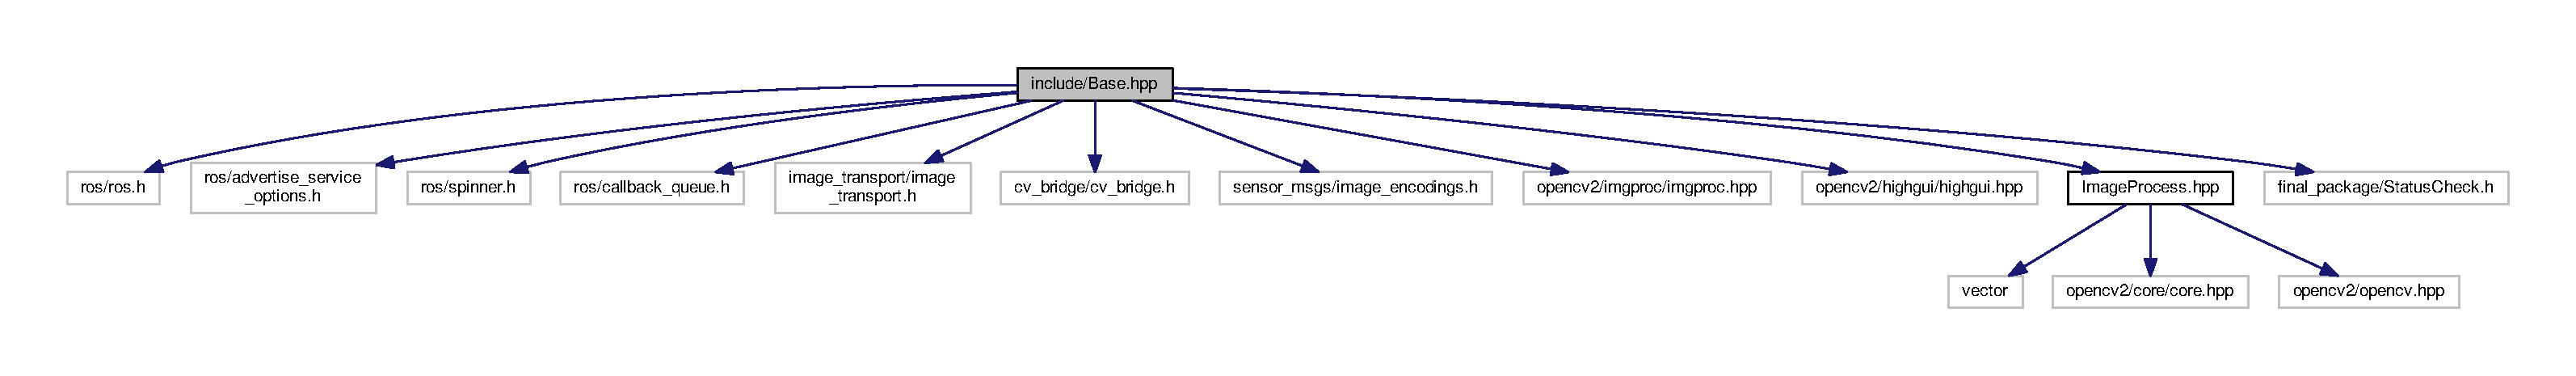
\includegraphics[width=350pt]{Base_8hpp__incl}
\end{center}
\end{figure}
This graph shows which files directly or indirectly include this file\+:\nopagebreak
\begin{figure}[H]
\begin{center}
\leavevmode
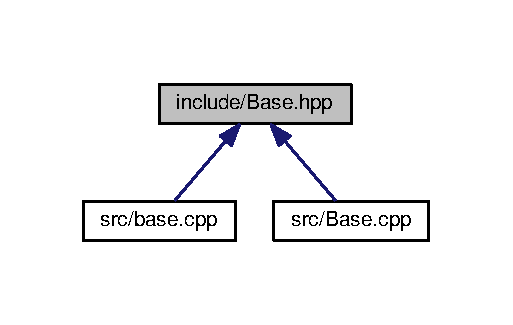
\includegraphics[width=246pt]{Base_8hpp__dep__incl}
\end{center}
\end{figure}
\subsection*{Classes}
\begin{DoxyCompactItemize}
\item 
class \hyperlink{classBase}{Base}
\end{DoxyCompactItemize}


\subsection{Detailed Description}
In this project, the nodes are being implemented as class objects. This is the header file for the base class. 

\begin{DoxyAuthor}{Author}
Yuyu Hsueh  2017, Yuyu Hsueh 
\end{DoxyAuthor}

\hypertarget{ImageProcess_8hpp}{}\section{include/\+Image\+Process.hpp File Reference}
\label{ImageProcess_8hpp}\index{include/\+Image\+Process.\+hpp@{include/\+Image\+Process.\+hpp}}


This is a header file for \hyperlink{classImageProcess}{Image\+Process} class, processing the images gotten from the 3D sensor.  


{\ttfamily \#include $<$vector$>$}\\*
{\ttfamily \#include $<$opencv2/core/core.\+hpp$>$}\\*
{\ttfamily \#include $<$opencv2/opencv.\+hpp$>$}\\*
Include dependency graph for Image\+Process.\+hpp\+:
\nopagebreak
\begin{figure}[H]
\begin{center}
\leavevmode
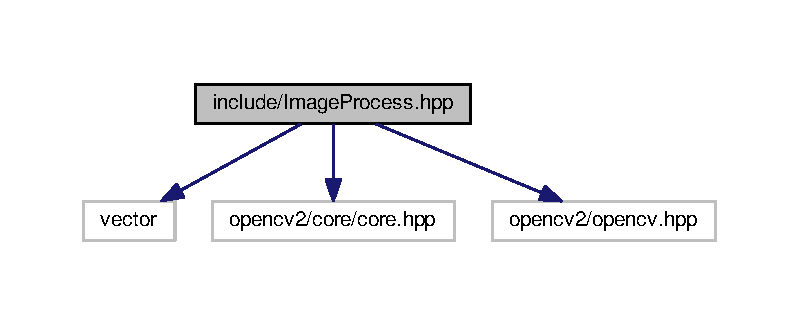
\includegraphics[width=350pt]{ImageProcess_8hpp__incl}
\end{center}
\end{figure}
This graph shows which files directly or indirectly include this file\+:
\nopagebreak
\begin{figure}[H]
\begin{center}
\leavevmode
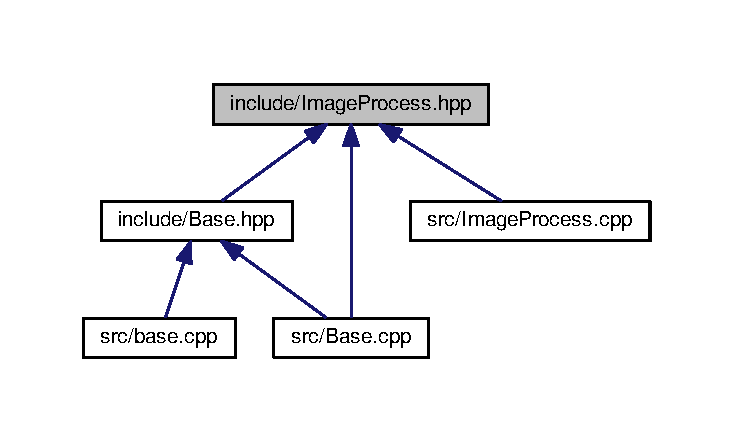
\includegraphics[width=350pt]{ImageProcess_8hpp__dep__incl}
\end{center}
\end{figure}
\subsection*{Classes}
\begin{DoxyCompactItemize}
\item 
class \hyperlink{classImageProcess}{Image\+Process}
\end{DoxyCompactItemize}


\subsection{Detailed Description}
This is a header file for \hyperlink{classImageProcess}{Image\+Process} class, processing the images gotten from the 3D sensor. 

\begin{DoxyAuthor}{Author}
Yuyu Hsueh  2017, Yuyu Hsueh 
\end{DoxyAuthor}

\hypertarget{TurtleCtrl_8hpp}{}\section{include/\+Turtle\+Ctrl.hpp File Reference}
\label{TurtleCtrl_8hpp}\index{include/\+Turtle\+Ctrl.\+hpp@{include/\+Turtle\+Ctrl.\+hpp}}


The turtlectrller node has been implemented as a class. It has multiple services and publisher/subscribers in order to drive the turtlebot toward the ball objects.  


{\ttfamily \#include $<$ros/ros.\+h$>$}\\*
{\ttfamily \#include $<$ros/spinner.\+h$>$}\\*
{\ttfamily \#include $<$ros/callback\+\_\+queue.\+h$>$}\\*
{\ttfamily \#include $<$ros/advertise\+\_\+service\+\_\+options.\+h$>$}\\*
{\ttfamily \#include \char`\"{}std\+\_\+msgs/\+Int64.\+h\char`\"{}}\\*
{\ttfamily \#include \char`\"{}geometry\+\_\+msgs/\+Twist.\+h\char`\"{}}\\*
{\ttfamily \#include \char`\"{}sensor\+\_\+msgs/\+Laser\+Scan.\+h\char`\"{}}\\*
{\ttfamily \#include \char`\"{}final\+\_\+package/\+Color\+Change.\+h\char`\"{}}\\*
Include dependency graph for Turtle\+Ctrl.\+hpp\+:
\nopagebreak
\begin{figure}[H]
\begin{center}
\leavevmode
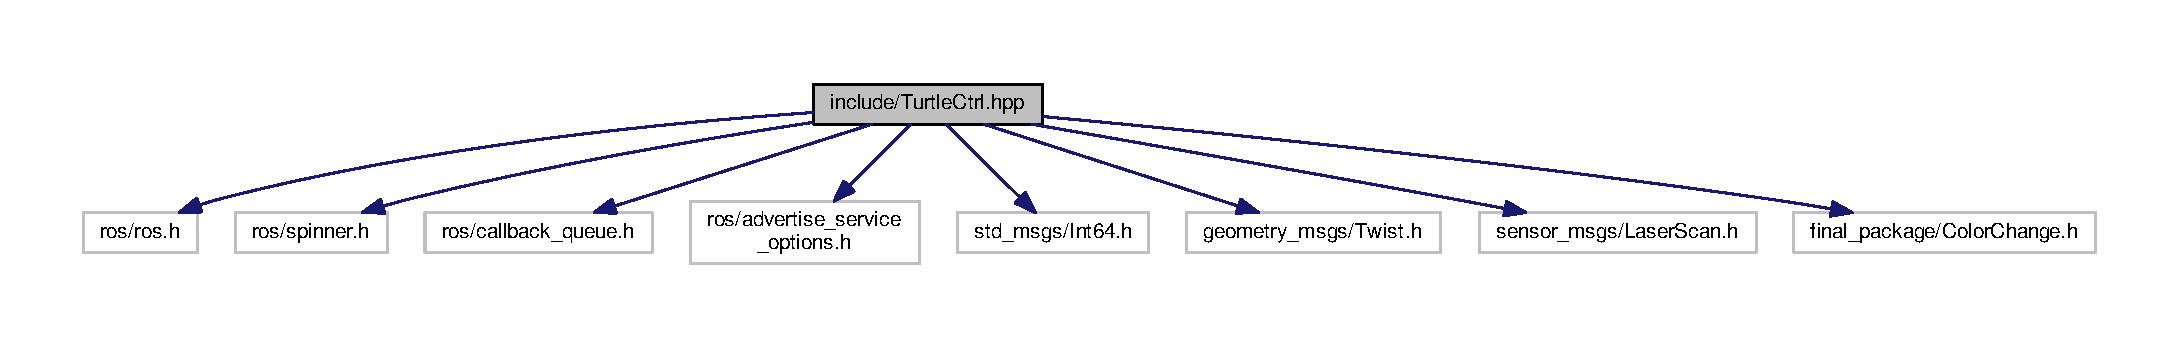
\includegraphics[width=350pt]{TurtleCtrl_8hpp__incl}
\end{center}
\end{figure}
This graph shows which files directly or indirectly include this file\+:
\nopagebreak
\begin{figure}[H]
\begin{center}
\leavevmode
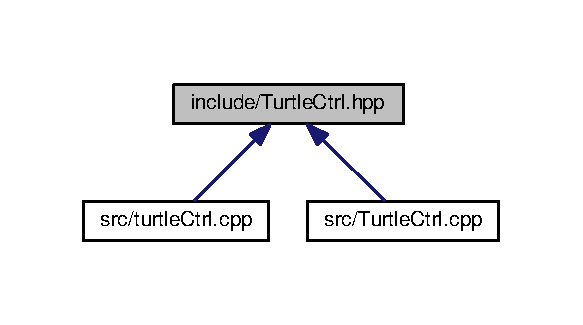
\includegraphics[width=280pt]{TurtleCtrl_8hpp__dep__incl}
\end{center}
\end{figure}
\subsection*{Classes}
\begin{DoxyCompactItemize}
\item 
class \hyperlink{classTurtleCtrl}{Turtle\+Ctrl}
\end{DoxyCompactItemize}


\subsection{Detailed Description}
The turtlectrller node has been implemented as a class. It has multiple services and publisher/subscribers in order to drive the turtlebot toward the ball objects. 

\begin{DoxyAuthor}{Author}
Yuyu Hsueh  2017, Yuyu Hsueh 
\end{DoxyAuthor}

\hypertarget{license_8txt}{}\section{license.\+txt File Reference}
\label{license_8txt}\index{license.\+txt@{license.\+txt}}
\subsection*{Functions}
\begin{DoxyCompactItemize}
\item 
Copyright Yuyu\+Hsueh Redistribution and use in source and binary with or without are permitted provided that the following conditions are this list of conditions and the following disclaimer Redistributions in binary form must reproduce the above copyright this list of conditions and the following disclaimer in the documentation and or other materials provided with the distribution Neither the name of the copyright holder nor the names of its contributors may be used to endorse or promote products derived from this software without specific prior written permission T\+H\+IS S\+O\+F\+T\+W\+A\+RE IS P\+R\+O\+V\+I\+D\+ED BY T\+HE C\+O\+P\+Y\+R\+I\+G\+HT H\+O\+L\+D\+E\+RS A\+ND C\+O\+N\+T\+R\+I\+B\+U\+T\+O\+RS AS IS A\+ND A\+NY E\+X\+P\+R\+E\+SS OR I\+M\+P\+L\+I\+ED B\+UT N\+OT L\+I\+M\+I\+T\+ED T\+HE I\+M\+P\+L\+I\+ED \hyperlink{license_8txt_a042eb66328050ad88743187ae8e43b95}{W\+A\+R\+R\+A\+N\+T\+I\+ES} OF M\+E\+R\+C\+H\+A\+N\+T\+A\+B\+I\+L\+I\+TY A\+ND F\+I\+T\+N\+E\+SS F\+OR A P\+A\+R\+T\+I\+C\+U\+L\+AR P\+U\+R\+P\+O\+SE A\+RE D\+I\+S\+C\+L\+A\+I\+M\+ED IN NO E\+V\+E\+NT S\+H\+A\+LL T\+HE C\+O\+P\+Y\+R\+I\+G\+HT H\+O\+L\+D\+ER OR C\+O\+N\+T\+R\+I\+B\+U\+T\+O\+RS BE L\+I\+A\+B\+LE F\+OR A\+NY OR C\+O\+N\+S\+E\+Q\+U\+E\+N\+T\+I\+AL \hyperlink{license_8txt_aef6a70d7e2ff0800bdd6b6c943108868}{D\+A\+M\+A\+G\+ES} (\hyperlink{license_8txt_ac6699313e23a90e93d8db75154e2e689}{I\+N\+C\+L\+U\+D\+I\+NG}, B\+UT N\+OT L\+I\+M\+I\+T\+ED \hyperlink{license_8txt_a4bddb9a7dc45727be85d1869ee6c870d}{TO}, P\+R\+O\+C\+U\+R\+E\+M\+E\+NT OF S\+U\+B\+S\+T\+I\+T\+U\+TE G\+O\+O\+DS OR S\+E\+R\+V\+I\+C\+ES;L\+O\+SS OF U\+SE, D\+A\+TA, OR P\+R\+O\+F\+I\+TS;OR B\+U\+S\+I\+N\+E\+SS I\+N\+T\+E\+R\+R\+U\+P\+T\+I\+ON) H\+O\+W\+E\+V\+ER C\+A\+U\+S\+ED A\+ND ON A\+NY T\+H\+E\+O\+RY OF \hyperlink{license_8txt_a293cddb201641aed1186322968630e55}{L\+I\+A\+B\+I\+L\+I\+TY}
\item 
Copyright Yuyu\+Hsueh Redistribution and use in source and binary with or without are permitted provided that the following conditions are this list of conditions and the following disclaimer Redistributions in binary form must reproduce the above copyright this list of conditions and the following disclaimer in the documentation and or other materials provided with the distribution Neither the name of the copyright holder nor the names of its contributors may be used to endorse or promote products derived from this software without specific prior written permission T\+H\+IS S\+O\+F\+T\+W\+A\+RE IS P\+R\+O\+V\+I\+D\+ED BY T\+HE C\+O\+P\+Y\+R\+I\+G\+HT H\+O\+L\+D\+E\+RS A\+ND C\+O\+N\+T\+R\+I\+B\+U\+T\+O\+RS AS IS A\+ND A\+NY E\+X\+P\+R\+E\+SS OR I\+M\+P\+L\+I\+ED B\+UT N\+OT L\+I\+M\+I\+T\+ED T\+HE I\+M\+P\+L\+I\+ED \hyperlink{license_8txt_a042eb66328050ad88743187ae8e43b95}{W\+A\+R\+R\+A\+N\+T\+I\+ES} OF M\+E\+R\+C\+H\+A\+N\+T\+A\+B\+I\+L\+I\+TY A\+ND F\+I\+T\+N\+E\+SS F\+OR A P\+A\+R\+T\+I\+C\+U\+L\+AR P\+U\+R\+P\+O\+SE A\+RE D\+I\+S\+C\+L\+A\+I\+M\+ED IN NO E\+V\+E\+NT S\+H\+A\+LL T\+HE C\+O\+P\+Y\+R\+I\+G\+HT H\+O\+L\+D\+ER OR C\+O\+N\+T\+R\+I\+B\+U\+T\+O\+RS BE L\+I\+A\+B\+LE F\+OR A\+NY OR C\+O\+N\+S\+E\+Q\+U\+E\+N\+T\+I\+AL W\+H\+E\+T\+H\+ER IN S\+T\+R\+I\+CT OR \hyperlink{license_8txt_a053f3866e9a0ed6d815ff119b776cf19}{T\+O\+RT} (\hyperlink{license_8txt_ac6699313e23a90e93d8db75154e2e689}{I\+N\+C\+L\+U\+D\+I\+NG} N\+E\+G\+L\+I\+G\+E\+N\+CE OR O\+T\+H\+E\+R\+W\+I\+SE) A\+R\+I\+S\+I\+NG IN A\+NY W\+AY O\+UT OF T\+HE U\+SE OF T\+H\+IS S\+O\+F\+T\+W\+A\+RE
\end{DoxyCompactItemize}
\subsection*{Variables}
\begin{DoxyCompactItemize}
\item 
Copyright Yuyu\+Hsueh Redistribution and use in source and binary \hyperlink{license_8txt_a907462b7b3ae0a9072f23e05f66fb7f1}{forms}
\item 
Copyright Yuyu\+Hsueh Redistribution and use in source and binary with or without \hyperlink{license_8txt_ad26192e5b2b1fdec8883d2c0110e35c6}{modification}
\item 
Copyright Yuyu\+Hsueh Redistribution and use in source and binary with or without are permitted provided that the following conditions are \hyperlink{license_8txt_ac8582a50364a60dd4d7d7d24f725c413}{met}
\item 
Copyright Yuyu\+Hsueh Redistribution and use in source and binary with or without are permitted provided that the following conditions are this list of conditions and the following disclaimer Redistributions in binary form must reproduce the above copyright \hyperlink{license_8txt_af4bbea5cb99610e4ef2a43c12b41e9c9}{notice}
\item 
Copyright Yuyu\+Hsueh Redistribution and use in source and binary with or without are permitted provided that the following conditions are this list of conditions and the following disclaimer Redistributions in binary form must reproduce the above copyright this list of conditions and the following disclaimer in the documentation and or other materials provided with the distribution Neither the name of the copyright holder nor the names of its contributors may be used to endorse or promote products derived from this software without specific prior written permission T\+H\+IS S\+O\+F\+T\+W\+A\+RE IS P\+R\+O\+V\+I\+D\+ED BY T\+HE C\+O\+P\+Y\+R\+I\+G\+HT H\+O\+L\+D\+E\+RS A\+ND C\+O\+N\+T\+R\+I\+B\+U\+T\+O\+RS AS IS A\+ND A\+NY E\+X\+P\+R\+E\+SS OR I\+M\+P\+L\+I\+ED \hyperlink{license_8txt_a042eb66328050ad88743187ae8e43b95}{W\+A\+R\+R\+A\+N\+T\+I\+ES}
\item 
Copyright Yuyu\+Hsueh Redistribution and use in source and binary with or without are permitted provided that the following conditions are this list of conditions and the following disclaimer Redistributions in binary form must reproduce the above copyright this list of conditions and the following disclaimer in the documentation and or other materials provided with the distribution Neither the name of the copyright holder nor the names of its contributors may be used to endorse or promote products derived from this software without specific prior written permission T\+H\+IS S\+O\+F\+T\+W\+A\+RE IS P\+R\+O\+V\+I\+D\+ED BY T\+HE C\+O\+P\+Y\+R\+I\+G\+HT H\+O\+L\+D\+E\+RS A\+ND C\+O\+N\+T\+R\+I\+B\+U\+T\+O\+RS AS IS A\+ND A\+NY E\+X\+P\+R\+E\+SS OR I\+M\+P\+L\+I\+ED \hyperlink{license_8txt_ac6699313e23a90e93d8db75154e2e689}{I\+N\+C\+L\+U\+D\+I\+NG}
\item 
Copyright Yuyu\+Hsueh Redistribution and use in source and binary with or without are permitted provided that the following conditions are this list of conditions and the following disclaimer Redistributions in binary form must reproduce the above copyright this list of conditions and the following disclaimer in the documentation and or other materials provided with the distribution Neither the name of the copyright holder nor the names of its contributors may be used to endorse or promote products derived from this software without specific prior written permission T\+H\+IS S\+O\+F\+T\+W\+A\+RE IS P\+R\+O\+V\+I\+D\+ED BY T\+HE C\+O\+P\+Y\+R\+I\+G\+HT H\+O\+L\+D\+E\+RS A\+ND C\+O\+N\+T\+R\+I\+B\+U\+T\+O\+RS AS IS A\+ND A\+NY E\+X\+P\+R\+E\+SS OR I\+M\+P\+L\+I\+ED B\+UT N\+OT L\+I\+M\+I\+T\+ED \hyperlink{license_8txt_a4bddb9a7dc45727be85d1869ee6c870d}{TO}
\item 
Copyright Yuyu\+Hsueh Redistribution and use in source and binary with or without are permitted provided that the following conditions are this list of conditions and the following disclaimer Redistributions in binary form must reproduce the above copyright this list of conditions and the following disclaimer in the documentation and or other materials provided with the distribution Neither the name of the copyright holder nor the names of its contributors may be used to endorse or promote products derived from this software without specific prior written permission T\+H\+IS S\+O\+F\+T\+W\+A\+RE IS P\+R\+O\+V\+I\+D\+ED BY T\+HE C\+O\+P\+Y\+R\+I\+G\+HT H\+O\+L\+D\+E\+RS A\+ND C\+O\+N\+T\+R\+I\+B\+U\+T\+O\+RS AS IS A\+ND A\+NY E\+X\+P\+R\+E\+SS OR I\+M\+P\+L\+I\+ED B\+UT N\+OT L\+I\+M\+I\+T\+ED T\+HE I\+M\+P\+L\+I\+ED \hyperlink{license_8txt_a042eb66328050ad88743187ae8e43b95}{W\+A\+R\+R\+A\+N\+T\+I\+ES} OF M\+E\+R\+C\+H\+A\+N\+T\+A\+B\+I\+L\+I\+TY A\+ND F\+I\+T\+N\+E\+SS F\+OR A P\+A\+R\+T\+I\+C\+U\+L\+AR P\+U\+R\+P\+O\+SE A\+RE D\+I\+S\+C\+L\+A\+I\+M\+ED IN NO E\+V\+E\+NT S\+H\+A\+LL T\+HE C\+O\+P\+Y\+R\+I\+G\+HT H\+O\+L\+D\+ER OR C\+O\+N\+T\+R\+I\+B\+U\+T\+O\+RS BE L\+I\+A\+B\+LE F\+OR A\+NY \hyperlink{license_8txt_a9ecfdaf89f3cf85421feb43ef16f372d}{D\+I\+R\+E\+CT}
\item 
Copyright Yuyu\+Hsueh Redistribution and use in source and binary with or without are permitted provided that the following conditions are this list of conditions and the following disclaimer Redistributions in binary form must reproduce the above copyright this list of conditions and the following disclaimer in the documentation and or other materials provided with the distribution Neither the name of the copyright holder nor the names of its contributors may be used to endorse or promote products derived from this software without specific prior written permission T\+H\+IS S\+O\+F\+T\+W\+A\+RE IS P\+R\+O\+V\+I\+D\+ED BY T\+HE C\+O\+P\+Y\+R\+I\+G\+HT H\+O\+L\+D\+E\+RS A\+ND C\+O\+N\+T\+R\+I\+B\+U\+T\+O\+RS AS IS A\+ND A\+NY E\+X\+P\+R\+E\+SS OR I\+M\+P\+L\+I\+ED B\+UT N\+OT L\+I\+M\+I\+T\+ED T\+HE I\+M\+P\+L\+I\+ED \hyperlink{license_8txt_a042eb66328050ad88743187ae8e43b95}{W\+A\+R\+R\+A\+N\+T\+I\+ES} OF M\+E\+R\+C\+H\+A\+N\+T\+A\+B\+I\+L\+I\+TY A\+ND F\+I\+T\+N\+E\+SS F\+OR A P\+A\+R\+T\+I\+C\+U\+L\+AR P\+U\+R\+P\+O\+SE A\+RE D\+I\+S\+C\+L\+A\+I\+M\+ED IN NO E\+V\+E\+NT S\+H\+A\+LL T\+HE C\+O\+P\+Y\+R\+I\+G\+HT H\+O\+L\+D\+ER OR C\+O\+N\+T\+R\+I\+B\+U\+T\+O\+RS BE L\+I\+A\+B\+LE F\+OR A\+NY \hyperlink{license_8txt_a8c44c311e30c2c13cd7035f237993b51}{I\+N\+D\+I\+R\+E\+CT}
\item 
Copyright Yuyu\+Hsueh Redistribution and use in source and binary with or without are permitted provided that the following conditions are this list of conditions and the following disclaimer Redistributions in binary form must reproduce the above copyright this list of conditions and the following disclaimer in the documentation and or other materials provided with the distribution Neither the name of the copyright holder nor the names of its contributors may be used to endorse or promote products derived from this software without specific prior written permission T\+H\+IS S\+O\+F\+T\+W\+A\+RE IS P\+R\+O\+V\+I\+D\+ED BY T\+HE C\+O\+P\+Y\+R\+I\+G\+HT H\+O\+L\+D\+E\+RS A\+ND C\+O\+N\+T\+R\+I\+B\+U\+T\+O\+RS AS IS A\+ND A\+NY E\+X\+P\+R\+E\+SS OR I\+M\+P\+L\+I\+ED B\+UT N\+OT L\+I\+M\+I\+T\+ED T\+HE I\+M\+P\+L\+I\+ED \hyperlink{license_8txt_a042eb66328050ad88743187ae8e43b95}{W\+A\+R\+R\+A\+N\+T\+I\+ES} OF M\+E\+R\+C\+H\+A\+N\+T\+A\+B\+I\+L\+I\+TY A\+ND F\+I\+T\+N\+E\+SS F\+OR A P\+A\+R\+T\+I\+C\+U\+L\+AR P\+U\+R\+P\+O\+SE A\+RE D\+I\+S\+C\+L\+A\+I\+M\+ED IN NO E\+V\+E\+NT S\+H\+A\+LL T\+HE C\+O\+P\+Y\+R\+I\+G\+HT H\+O\+L\+D\+ER OR C\+O\+N\+T\+R\+I\+B\+U\+T\+O\+RS BE L\+I\+A\+B\+LE F\+OR A\+NY \hyperlink{license_8txt_a6fe13299500a9a6c4af4434723e6afae}{I\+N\+C\+I\+D\+E\+N\+T\+AL}
\item 
Copyright Yuyu\+Hsueh Redistribution and use in source and binary with or without are permitted provided that the following conditions are this list of conditions and the following disclaimer Redistributions in binary form must reproduce the above copyright this list of conditions and the following disclaimer in the documentation and or other materials provided with the distribution Neither the name of the copyright holder nor the names of its contributors may be used to endorse or promote products derived from this software without specific prior written permission T\+H\+IS S\+O\+F\+T\+W\+A\+RE IS P\+R\+O\+V\+I\+D\+ED BY T\+HE C\+O\+P\+Y\+R\+I\+G\+HT H\+O\+L\+D\+E\+RS A\+ND C\+O\+N\+T\+R\+I\+B\+U\+T\+O\+RS AS IS A\+ND A\+NY E\+X\+P\+R\+E\+SS OR I\+M\+P\+L\+I\+ED B\+UT N\+OT L\+I\+M\+I\+T\+ED T\+HE I\+M\+P\+L\+I\+ED \hyperlink{license_8txt_a042eb66328050ad88743187ae8e43b95}{W\+A\+R\+R\+A\+N\+T\+I\+ES} OF M\+E\+R\+C\+H\+A\+N\+T\+A\+B\+I\+L\+I\+TY A\+ND F\+I\+T\+N\+E\+SS F\+OR A P\+A\+R\+T\+I\+C\+U\+L\+AR P\+U\+R\+P\+O\+SE A\+RE D\+I\+S\+C\+L\+A\+I\+M\+ED IN NO E\+V\+E\+NT S\+H\+A\+LL T\+HE C\+O\+P\+Y\+R\+I\+G\+HT H\+O\+L\+D\+ER OR C\+O\+N\+T\+R\+I\+B\+U\+T\+O\+RS BE L\+I\+A\+B\+LE F\+OR A\+NY \hyperlink{license_8txt_a910ad17f295c48bc77c8ee2434bf4ac5}{S\+P\+E\+C\+I\+AL}
\item 
Copyright Yuyu\+Hsueh Redistribution and use in source and binary with or without are permitted provided that the following conditions are this list of conditions and the following disclaimer Redistributions in binary form must reproduce the above copyright this list of conditions and the following disclaimer in the documentation and or other materials provided with the distribution Neither the name of the copyright holder nor the names of its contributors may be used to endorse or promote products derived from this software without specific prior written permission T\+H\+IS S\+O\+F\+T\+W\+A\+RE IS P\+R\+O\+V\+I\+D\+ED BY T\+HE C\+O\+P\+Y\+R\+I\+G\+HT H\+O\+L\+D\+E\+RS A\+ND C\+O\+N\+T\+R\+I\+B\+U\+T\+O\+RS AS IS A\+ND A\+NY E\+X\+P\+R\+E\+SS OR I\+M\+P\+L\+I\+ED B\+UT N\+OT L\+I\+M\+I\+T\+ED T\+HE I\+M\+P\+L\+I\+ED \hyperlink{license_8txt_a042eb66328050ad88743187ae8e43b95}{W\+A\+R\+R\+A\+N\+T\+I\+ES} OF M\+E\+R\+C\+H\+A\+N\+T\+A\+B\+I\+L\+I\+TY A\+ND F\+I\+T\+N\+E\+SS F\+OR A P\+A\+R\+T\+I\+C\+U\+L\+AR P\+U\+R\+P\+O\+SE A\+RE D\+I\+S\+C\+L\+A\+I\+M\+ED IN NO E\+V\+E\+NT S\+H\+A\+LL T\+HE C\+O\+P\+Y\+R\+I\+G\+HT H\+O\+L\+D\+ER OR C\+O\+N\+T\+R\+I\+B\+U\+T\+O\+RS BE L\+I\+A\+B\+LE F\+OR A\+NY \hyperlink{license_8txt_ac4a6acd1ced6bfbf36f00e4629d74515}{E\+X\+E\+M\+P\+L\+A\+RY}
\item 
Copyright Yuyu\+Hsueh Redistribution and use in source and binary with or without are permitted provided that the following conditions are this list of conditions and the following disclaimer Redistributions in binary form must reproduce the above copyright this list of conditions and the following disclaimer in the documentation and or other materials provided with the distribution Neither the name of the copyright holder nor the names of its contributors may be used to endorse or promote products derived from this software without specific prior written permission T\+H\+IS S\+O\+F\+T\+W\+A\+RE IS P\+R\+O\+V\+I\+D\+ED BY T\+HE C\+O\+P\+Y\+R\+I\+G\+HT H\+O\+L\+D\+E\+RS A\+ND C\+O\+N\+T\+R\+I\+B\+U\+T\+O\+RS AS IS A\+ND A\+NY E\+X\+P\+R\+E\+SS OR I\+M\+P\+L\+I\+ED B\+UT N\+OT L\+I\+M\+I\+T\+ED T\+HE I\+M\+P\+L\+I\+ED \hyperlink{license_8txt_a042eb66328050ad88743187ae8e43b95}{W\+A\+R\+R\+A\+N\+T\+I\+ES} OF M\+E\+R\+C\+H\+A\+N\+T\+A\+B\+I\+L\+I\+TY A\+ND F\+I\+T\+N\+E\+SS F\+OR A P\+A\+R\+T\+I\+C\+U\+L\+AR P\+U\+R\+P\+O\+SE A\+RE D\+I\+S\+C\+L\+A\+I\+M\+ED IN NO E\+V\+E\+NT S\+H\+A\+LL T\+HE C\+O\+P\+Y\+R\+I\+G\+HT H\+O\+L\+D\+ER OR C\+O\+N\+T\+R\+I\+B\+U\+T\+O\+RS BE L\+I\+A\+B\+LE F\+OR A\+NY OR C\+O\+N\+S\+E\+Q\+U\+E\+N\+T\+I\+AL W\+H\+E\+T\+H\+ER IN \hyperlink{license_8txt_ad1b3910f726d03f8987a2ad1665d309c}{C\+O\+N\+T\+R\+A\+CT}
\item 
Copyright Yuyu\+Hsueh Redistribution and use in source and binary with or without are permitted provided that the following conditions are this list of conditions and the following disclaimer Redistributions in binary form must reproduce the above copyright this list of conditions and the following disclaimer in the documentation and or other materials provided with the distribution Neither the name of the copyright holder nor the names of its contributors may be used to endorse or promote products derived from this software without specific prior written permission T\+H\+IS S\+O\+F\+T\+W\+A\+RE IS P\+R\+O\+V\+I\+D\+ED BY T\+HE C\+O\+P\+Y\+R\+I\+G\+HT H\+O\+L\+D\+E\+RS A\+ND C\+O\+N\+T\+R\+I\+B\+U\+T\+O\+RS AS IS A\+ND A\+NY E\+X\+P\+R\+E\+SS OR I\+M\+P\+L\+I\+ED B\+UT N\+OT L\+I\+M\+I\+T\+ED T\+HE I\+M\+P\+L\+I\+ED \hyperlink{license_8txt_a042eb66328050ad88743187ae8e43b95}{W\+A\+R\+R\+A\+N\+T\+I\+ES} OF M\+E\+R\+C\+H\+A\+N\+T\+A\+B\+I\+L\+I\+TY A\+ND F\+I\+T\+N\+E\+SS F\+OR A P\+A\+R\+T\+I\+C\+U\+L\+AR P\+U\+R\+P\+O\+SE A\+RE D\+I\+S\+C\+L\+A\+I\+M\+ED IN NO E\+V\+E\+NT S\+H\+A\+LL T\+HE C\+O\+P\+Y\+R\+I\+G\+HT H\+O\+L\+D\+ER OR C\+O\+N\+T\+R\+I\+B\+U\+T\+O\+RS BE L\+I\+A\+B\+LE F\+OR A\+NY OR C\+O\+N\+S\+E\+Q\+U\+E\+N\+T\+I\+AL W\+H\+E\+T\+H\+ER IN S\+T\+R\+I\+CT \hyperlink{license_8txt_a293cddb201641aed1186322968630e55}{L\+I\+A\+B\+I\+L\+I\+TY}
\end{DoxyCompactItemize}


\subsection{Function Documentation}
\index{license.\+txt@{license.\+txt}!D\+A\+M\+A\+G\+ES@{D\+A\+M\+A\+G\+ES}}
\index{D\+A\+M\+A\+G\+ES@{D\+A\+M\+A\+G\+ES}!license.\+txt@{license.\+txt}}
\subsubsection[{\texorpdfstring{D\+A\+M\+A\+G\+E\+S(\+I\+N\+C\+L\+U\+D\+I\+N\+G, B\+U\+T N\+O\+T L\+I\+M\+I\+T\+E\+D T\+O, P\+R\+O\+C\+U\+R\+E\+M\+E\+N\+T O\+F S\+U\+B\+S\+T\+I\+T\+U\+T\+E G\+O\+O\+D\+S O\+R S\+E\+R\+V\+I\+C\+E\+S;\+L\+O\+S\+S O\+F U\+S\+E, D\+A\+T\+A, O\+R P\+R\+O\+F\+I\+T\+S;\+O\+R B\+U\+S\+I\+N\+E\+S\+S I\+N\+T\+E\+R\+R\+U\+P\+T\+I\+O\+N) H\+O\+W\+E\+V\+E\+R C\+A\+U\+S\+E\+D A\+N\+D O\+N A\+N\+Y T\+H\+E\+O\+R\+Y O\+F L\+I\+A\+B\+I\+L\+I\+TY}{DAMAGES(INCLUDING, BUT NOT LIMITED TO, PROCUREMENT OF SUBSTITUTE GOODS OR SERVICES;LOSS OF USE, DATA, OR PROFITS;OR BUSINESS INTERRUPTION) HOWEVER CAUSED AND ON ANY THEORY OF LIABILITY}}]{\setlength{\rightskip}{0pt plus 5cm}Copyright Yuyu\+Hsueh Redistribution and use in source and binary with or without are permitted provided that the following conditions are this list of conditions and the following disclaimer Redistributions in binary form must reproduce the above copyright this list of conditions and the following disclaimer in the documentation and or other materials provided with the distribution Neither the name of the copyright holder nor the names of its contributors may be used to endorse or promote products derived from this software without specific prior written permission T\+H\+IS S\+O\+F\+T\+W\+A\+RE IS P\+R\+O\+V\+I\+D\+ED BY T\+HE C\+O\+P\+Y\+R\+I\+G\+HT H\+O\+L\+D\+E\+RS A\+ND C\+O\+N\+T\+R\+I\+B\+U\+T\+O\+RS AS IS A\+ND A\+NY E\+X\+P\+R\+E\+SS OR I\+M\+P\+L\+I\+ED B\+UT N\+OT L\+I\+M\+I\+T\+ED T\+HE I\+M\+P\+L\+I\+ED {\bf W\+A\+R\+R\+A\+N\+T\+I\+ES} OF M\+E\+R\+C\+H\+A\+N\+T\+A\+B\+I\+L\+I\+TY A\+ND F\+I\+T\+N\+E\+SS F\+OR A P\+A\+R\+T\+I\+C\+U\+L\+AR P\+U\+R\+P\+O\+SE A\+RE D\+I\+S\+C\+L\+A\+I\+M\+ED IN NO E\+V\+E\+NT S\+H\+A\+LL T\+HE C\+O\+P\+Y\+R\+I\+G\+HT H\+O\+L\+D\+ER OR C\+O\+N\+T\+R\+I\+B\+U\+T\+O\+RS BE L\+I\+A\+B\+LE F\+OR A\+NY OR C\+O\+N\+S\+E\+Q\+U\+E\+N\+T\+I\+AL D\+A\+M\+A\+G\+ES (
\begin{DoxyParamCaption}
\item[{{\bf I\+N\+C\+L\+U\+D\+I\+NG}}]{, }
\item[{B\+UT N\+OT L\+I\+M\+I\+T\+ED}]{TO, }
\item[{P\+R\+O\+C\+U\+R\+E\+M\+E\+NT OF S\+U\+B\+S\+T\+I\+T\+U\+TE G\+O\+O\+DS OR S\+E\+R\+V\+I\+C\+ES;L\+O\+SS OF}]{U\+SE, }
\item[{D\+A\+TA}]{, }
\item[{OR P\+R\+O\+F\+I\+TS;OR B\+U\+S\+I\+N\+E\+SS}]{I\+N\+T\+E\+R\+R\+U\+P\+T\+I\+ON}
\end{DoxyParamCaption}
)}\hypertarget{license_8txt_aef6a70d7e2ff0800bdd6b6c943108868}{}\label{license_8txt_aef6a70d7e2ff0800bdd6b6c943108868}
\index{license.\+txt@{license.\+txt}!T\+O\+RT@{T\+O\+RT}}
\index{T\+O\+RT@{T\+O\+RT}!license.\+txt@{license.\+txt}}
\subsubsection[{\texorpdfstring{T\+O\+R\+T(\+I\+N\+C\+L\+U\+D\+I\+N\+G N\+E\+G\+L\+I\+G\+E\+N\+C\+E O\+R O\+T\+H\+E\+R\+W\+I\+S\+E) A\+R\+I\+S\+I\+N\+G I\+N A\+N\+Y W\+A\+Y O\+U\+T O\+F T\+H\+E U\+S\+E O\+F T\+H\+I\+S S\+O\+F\+T\+W\+A\+RE}{TORT(INCLUDING NEGLIGENCE OR OTHERWISE) ARISING IN ANY WAY OUT OF THE USE OF THIS SOFTWARE}}]{\setlength{\rightskip}{0pt plus 5cm}Copyright Yuyu\+Hsueh Redistribution and use in source and binary with or without are permitted provided that the following conditions are this list of conditions and the following disclaimer Redistributions in binary form must reproduce the above copyright this list of conditions and the following disclaimer in the documentation and or other materials provided with the distribution Neither the name of the copyright holder nor the names of its contributors may be used to endorse or promote products derived from this software without specific prior written permission T\+H\+IS S\+O\+F\+T\+W\+A\+RE IS P\+R\+O\+V\+I\+D\+ED BY T\+HE C\+O\+P\+Y\+R\+I\+G\+HT H\+O\+L\+D\+E\+RS A\+ND C\+O\+N\+T\+R\+I\+B\+U\+T\+O\+RS AS IS A\+ND A\+NY E\+X\+P\+R\+E\+SS OR I\+M\+P\+L\+I\+ED B\+UT N\+OT L\+I\+M\+I\+T\+ED T\+HE I\+M\+P\+L\+I\+ED {\bf W\+A\+R\+R\+A\+N\+T\+I\+ES} OF M\+E\+R\+C\+H\+A\+N\+T\+A\+B\+I\+L\+I\+TY A\+ND F\+I\+T\+N\+E\+SS F\+OR A P\+A\+R\+T\+I\+C\+U\+L\+AR P\+U\+R\+P\+O\+SE A\+RE D\+I\+S\+C\+L\+A\+I\+M\+ED IN NO E\+V\+E\+NT S\+H\+A\+LL T\+HE C\+O\+P\+Y\+R\+I\+G\+HT H\+O\+L\+D\+ER OR C\+O\+N\+T\+R\+I\+B\+U\+T\+O\+RS BE L\+I\+A\+B\+LE F\+OR A\+NY OR C\+O\+N\+S\+E\+Q\+U\+E\+N\+T\+I\+AL W\+H\+E\+T\+H\+ER IN S\+T\+R\+I\+CT OR T\+O\+RT (
\begin{DoxyParamCaption}
\item[{{\bf I\+N\+C\+L\+U\+D\+I\+NG} N\+E\+G\+L\+I\+G\+E\+N\+CE OR}]{O\+T\+H\+E\+R\+W\+I\+SE}
\end{DoxyParamCaption}
)}\hypertarget{license_8txt_a053f3866e9a0ed6d815ff119b776cf19}{}\label{license_8txt_a053f3866e9a0ed6d815ff119b776cf19}


\subsection{Variable Documentation}
\index{license.\+txt@{license.\+txt}!C\+O\+N\+T\+R\+A\+CT@{C\+O\+N\+T\+R\+A\+CT}}
\index{C\+O\+N\+T\+R\+A\+CT@{C\+O\+N\+T\+R\+A\+CT}!license.\+txt@{license.\+txt}}
\subsubsection[{\texorpdfstring{C\+O\+N\+T\+R\+A\+CT}{CONTRACT}}]{\setlength{\rightskip}{0pt plus 5cm}Copyright Yuyu\+Hsueh Redistribution and use in source and binary with or without are permitted provided that the following conditions are this list of conditions and the following disclaimer Redistributions in binary form must reproduce the above copyright this list of conditions and the following disclaimer in the documentation and or other materials provided with the distribution Neither the name of the copyright holder nor the names of its contributors may be used to endorse or promote products derived from this software without specific prior written permission T\+H\+IS S\+O\+F\+T\+W\+A\+RE IS P\+R\+O\+V\+I\+D\+ED BY T\+HE C\+O\+P\+Y\+R\+I\+G\+HT H\+O\+L\+D\+E\+RS A\+ND C\+O\+N\+T\+R\+I\+B\+U\+T\+O\+RS AS IS A\+ND A\+NY E\+X\+P\+R\+E\+SS OR I\+M\+P\+L\+I\+ED B\+UT N\+OT L\+I\+M\+I\+T\+ED T\+HE I\+M\+P\+L\+I\+ED {\bf W\+A\+R\+R\+A\+N\+T\+I\+ES} OF M\+E\+R\+C\+H\+A\+N\+T\+A\+B\+I\+L\+I\+TY A\+ND F\+I\+T\+N\+E\+SS F\+OR A P\+A\+R\+T\+I\+C\+U\+L\+AR P\+U\+R\+P\+O\+SE A\+RE D\+I\+S\+C\+L\+A\+I\+M\+ED IN NO E\+V\+E\+NT S\+H\+A\+LL T\+HE C\+O\+P\+Y\+R\+I\+G\+HT H\+O\+L\+D\+ER OR C\+O\+N\+T\+R\+I\+B\+U\+T\+O\+RS BE L\+I\+A\+B\+LE F\+OR A\+NY OR C\+O\+N\+S\+E\+Q\+U\+E\+N\+T\+I\+AL W\+H\+E\+T\+H\+ER IN C\+O\+N\+T\+R\+A\+CT}\hypertarget{license_8txt_ad1b3910f726d03f8987a2ad1665d309c}{}\label{license_8txt_ad1b3910f726d03f8987a2ad1665d309c}
\index{license.\+txt@{license.\+txt}!D\+I\+R\+E\+CT@{D\+I\+R\+E\+CT}}
\index{D\+I\+R\+E\+CT@{D\+I\+R\+E\+CT}!license.\+txt@{license.\+txt}}
\subsubsection[{\texorpdfstring{D\+I\+R\+E\+CT}{DIRECT}}]{\setlength{\rightskip}{0pt plus 5cm}Copyright Yuyu\+Hsueh Redistribution and use in source and binary with or without are permitted provided that the following conditions are this list of conditions and the following disclaimer Redistributions in binary form must reproduce the above copyright this list of conditions and the following disclaimer in the documentation and or other materials provided with the distribution Neither the name of the copyright holder nor the names of its contributors may be used to endorse or promote products derived from this software without specific prior written permission T\+H\+IS S\+O\+F\+T\+W\+A\+RE IS P\+R\+O\+V\+I\+D\+ED BY T\+HE C\+O\+P\+Y\+R\+I\+G\+HT H\+O\+L\+D\+E\+RS A\+ND C\+O\+N\+T\+R\+I\+B\+U\+T\+O\+RS AS IS A\+ND A\+NY E\+X\+P\+R\+E\+SS OR I\+M\+P\+L\+I\+ED B\+UT N\+OT L\+I\+M\+I\+T\+ED T\+HE I\+M\+P\+L\+I\+ED {\bf W\+A\+R\+R\+A\+N\+T\+I\+ES} OF M\+E\+R\+C\+H\+A\+N\+T\+A\+B\+I\+L\+I\+TY A\+ND F\+I\+T\+N\+E\+SS F\+OR A P\+A\+R\+T\+I\+C\+U\+L\+AR P\+U\+R\+P\+O\+SE A\+RE D\+I\+S\+C\+L\+A\+I\+M\+ED IN NO E\+V\+E\+NT S\+H\+A\+LL T\+HE C\+O\+P\+Y\+R\+I\+G\+HT H\+O\+L\+D\+ER OR C\+O\+N\+T\+R\+I\+B\+U\+T\+O\+RS BE L\+I\+A\+B\+LE F\+OR A\+NY D\+I\+R\+E\+CT}\hypertarget{license_8txt_a9ecfdaf89f3cf85421feb43ef16f372d}{}\label{license_8txt_a9ecfdaf89f3cf85421feb43ef16f372d}
\index{license.\+txt@{license.\+txt}!E\+X\+E\+M\+P\+L\+A\+RY@{E\+X\+E\+M\+P\+L\+A\+RY}}
\index{E\+X\+E\+M\+P\+L\+A\+RY@{E\+X\+E\+M\+P\+L\+A\+RY}!license.\+txt@{license.\+txt}}
\subsubsection[{\texorpdfstring{E\+X\+E\+M\+P\+L\+A\+RY}{EXEMPLARY}}]{\setlength{\rightskip}{0pt plus 5cm}Copyright Yuyu\+Hsueh Redistribution and use in source and binary with or without are permitted provided that the following conditions are this list of conditions and the following disclaimer Redistributions in binary form must reproduce the above copyright this list of conditions and the following disclaimer in the documentation and or other materials provided with the distribution Neither the name of the copyright holder nor the names of its contributors may be used to endorse or promote products derived from this software without specific prior written permission T\+H\+IS S\+O\+F\+T\+W\+A\+RE IS P\+R\+O\+V\+I\+D\+ED BY T\+HE C\+O\+P\+Y\+R\+I\+G\+HT H\+O\+L\+D\+E\+RS A\+ND C\+O\+N\+T\+R\+I\+B\+U\+T\+O\+RS AS IS A\+ND A\+NY E\+X\+P\+R\+E\+SS OR I\+M\+P\+L\+I\+ED B\+UT N\+OT L\+I\+M\+I\+T\+ED T\+HE I\+M\+P\+L\+I\+ED {\bf W\+A\+R\+R\+A\+N\+T\+I\+ES} OF M\+E\+R\+C\+H\+A\+N\+T\+A\+B\+I\+L\+I\+TY A\+ND F\+I\+T\+N\+E\+SS F\+OR A P\+A\+R\+T\+I\+C\+U\+L\+AR P\+U\+R\+P\+O\+SE A\+RE D\+I\+S\+C\+L\+A\+I\+M\+ED IN NO E\+V\+E\+NT S\+H\+A\+LL T\+HE C\+O\+P\+Y\+R\+I\+G\+HT H\+O\+L\+D\+ER OR C\+O\+N\+T\+R\+I\+B\+U\+T\+O\+RS BE L\+I\+A\+B\+LE F\+OR A\+NY E\+X\+E\+M\+P\+L\+A\+RY}\hypertarget{license_8txt_ac4a6acd1ced6bfbf36f00e4629d74515}{}\label{license_8txt_ac4a6acd1ced6bfbf36f00e4629d74515}
\index{license.\+txt@{license.\+txt}!forms@{forms}}
\index{forms@{forms}!license.\+txt@{license.\+txt}}
\subsubsection[{\texorpdfstring{forms}{forms}}]{\setlength{\rightskip}{0pt plus 5cm}Copyright Yuyu\+Hsueh Redistribution and use in source and binary forms}\hypertarget{license_8txt_a907462b7b3ae0a9072f23e05f66fb7f1}{}\label{license_8txt_a907462b7b3ae0a9072f23e05f66fb7f1}
\index{license.\+txt@{license.\+txt}!I\+N\+C\+I\+D\+E\+N\+T\+AL@{I\+N\+C\+I\+D\+E\+N\+T\+AL}}
\index{I\+N\+C\+I\+D\+E\+N\+T\+AL@{I\+N\+C\+I\+D\+E\+N\+T\+AL}!license.\+txt@{license.\+txt}}
\subsubsection[{\texorpdfstring{I\+N\+C\+I\+D\+E\+N\+T\+AL}{INCIDENTAL}}]{\setlength{\rightskip}{0pt plus 5cm}Copyright Yuyu\+Hsueh Redistribution and use in source and binary with or without are permitted provided that the following conditions are this list of conditions and the following disclaimer Redistributions in binary form must reproduce the above copyright this list of conditions and the following disclaimer in the documentation and or other materials provided with the distribution Neither the name of the copyright holder nor the names of its contributors may be used to endorse or promote products derived from this software without specific prior written permission T\+H\+IS S\+O\+F\+T\+W\+A\+RE IS P\+R\+O\+V\+I\+D\+ED BY T\+HE C\+O\+P\+Y\+R\+I\+G\+HT H\+O\+L\+D\+E\+RS A\+ND C\+O\+N\+T\+R\+I\+B\+U\+T\+O\+RS AS IS A\+ND A\+NY E\+X\+P\+R\+E\+SS OR I\+M\+P\+L\+I\+ED B\+UT N\+OT L\+I\+M\+I\+T\+ED T\+HE I\+M\+P\+L\+I\+ED {\bf W\+A\+R\+R\+A\+N\+T\+I\+ES} OF M\+E\+R\+C\+H\+A\+N\+T\+A\+B\+I\+L\+I\+TY A\+ND F\+I\+T\+N\+E\+SS F\+OR A P\+A\+R\+T\+I\+C\+U\+L\+AR P\+U\+R\+P\+O\+SE A\+RE D\+I\+S\+C\+L\+A\+I\+M\+ED IN NO E\+V\+E\+NT S\+H\+A\+LL T\+HE C\+O\+P\+Y\+R\+I\+G\+HT H\+O\+L\+D\+ER OR C\+O\+N\+T\+R\+I\+B\+U\+T\+O\+RS BE L\+I\+A\+B\+LE F\+OR A\+NY I\+N\+C\+I\+D\+E\+N\+T\+AL}\hypertarget{license_8txt_a6fe13299500a9a6c4af4434723e6afae}{}\label{license_8txt_a6fe13299500a9a6c4af4434723e6afae}
\index{license.\+txt@{license.\+txt}!I\+N\+C\+L\+U\+D\+I\+NG@{I\+N\+C\+L\+U\+D\+I\+NG}}
\index{I\+N\+C\+L\+U\+D\+I\+NG@{I\+N\+C\+L\+U\+D\+I\+NG}!license.\+txt@{license.\+txt}}
\subsubsection[{\texorpdfstring{I\+N\+C\+L\+U\+D\+I\+NG}{INCLUDING}}]{\setlength{\rightskip}{0pt plus 5cm}Copyright Yuyu\+Hsueh Redistribution and use in source and binary with or without are permitted provided that the following conditions are this list of conditions and the following disclaimer Redistributions in binary form must reproduce the above copyright this list of conditions and the following disclaimer in the documentation and or other materials provided with the distribution Neither the name of the copyright holder nor the names of its contributors may be used to endorse or promote products derived from this software without specific prior written permission T\+H\+IS S\+O\+F\+T\+W\+A\+RE IS P\+R\+O\+V\+I\+D\+ED BY T\+HE C\+O\+P\+Y\+R\+I\+G\+HT H\+O\+L\+D\+E\+RS A\+ND C\+O\+N\+T\+R\+I\+B\+U\+T\+O\+RS AS IS A\+ND A\+NY E\+X\+P\+R\+E\+SS OR I\+M\+P\+L\+I\+ED I\+N\+C\+L\+U\+D\+I\+NG}\hypertarget{license_8txt_ac6699313e23a90e93d8db75154e2e689}{}\label{license_8txt_ac6699313e23a90e93d8db75154e2e689}
\index{license.\+txt@{license.\+txt}!I\+N\+D\+I\+R\+E\+CT@{I\+N\+D\+I\+R\+E\+CT}}
\index{I\+N\+D\+I\+R\+E\+CT@{I\+N\+D\+I\+R\+E\+CT}!license.\+txt@{license.\+txt}}
\subsubsection[{\texorpdfstring{I\+N\+D\+I\+R\+E\+CT}{INDIRECT}}]{\setlength{\rightskip}{0pt plus 5cm}Copyright Yuyu\+Hsueh Redistribution and use in source and binary with or without are permitted provided that the following conditions are this list of conditions and the following disclaimer Redistributions in binary form must reproduce the above copyright this list of conditions and the following disclaimer in the documentation and or other materials provided with the distribution Neither the name of the copyright holder nor the names of its contributors may be used to endorse or promote products derived from this software without specific prior written permission T\+H\+IS S\+O\+F\+T\+W\+A\+RE IS P\+R\+O\+V\+I\+D\+ED BY T\+HE C\+O\+P\+Y\+R\+I\+G\+HT H\+O\+L\+D\+E\+RS A\+ND C\+O\+N\+T\+R\+I\+B\+U\+T\+O\+RS AS IS A\+ND A\+NY E\+X\+P\+R\+E\+SS OR I\+M\+P\+L\+I\+ED B\+UT N\+OT L\+I\+M\+I\+T\+ED T\+HE I\+M\+P\+L\+I\+ED {\bf W\+A\+R\+R\+A\+N\+T\+I\+ES} OF M\+E\+R\+C\+H\+A\+N\+T\+A\+B\+I\+L\+I\+TY A\+ND F\+I\+T\+N\+E\+SS F\+OR A P\+A\+R\+T\+I\+C\+U\+L\+AR P\+U\+R\+P\+O\+SE A\+RE D\+I\+S\+C\+L\+A\+I\+M\+ED IN NO E\+V\+E\+NT S\+H\+A\+LL T\+HE C\+O\+P\+Y\+R\+I\+G\+HT H\+O\+L\+D\+ER OR C\+O\+N\+T\+R\+I\+B\+U\+T\+O\+RS BE L\+I\+A\+B\+LE F\+OR A\+NY I\+N\+D\+I\+R\+E\+CT}\hypertarget{license_8txt_a8c44c311e30c2c13cd7035f237993b51}{}\label{license_8txt_a8c44c311e30c2c13cd7035f237993b51}
\index{license.\+txt@{license.\+txt}!L\+I\+A\+B\+I\+L\+I\+TY@{L\+I\+A\+B\+I\+L\+I\+TY}}
\index{L\+I\+A\+B\+I\+L\+I\+TY@{L\+I\+A\+B\+I\+L\+I\+TY}!license.\+txt@{license.\+txt}}
\subsubsection[{\texorpdfstring{L\+I\+A\+B\+I\+L\+I\+TY}{LIABILITY}}]{\setlength{\rightskip}{0pt plus 5cm}Copyright Yuyu\+Hsueh Redistribution and use in source and binary with or without are permitted provided that the following conditions are this list of conditions and the following disclaimer Redistributions in binary form must reproduce the above copyright this list of conditions and the following disclaimer in the documentation and or other materials provided with the distribution Neither the name of the copyright holder nor the names of its contributors may be used to endorse or promote products derived from this software without specific prior written permission T\+H\+IS S\+O\+F\+T\+W\+A\+RE IS P\+R\+O\+V\+I\+D\+ED BY T\+HE C\+O\+P\+Y\+R\+I\+G\+HT H\+O\+L\+D\+E\+RS A\+ND C\+O\+N\+T\+R\+I\+B\+U\+T\+O\+RS AS IS A\+ND A\+NY E\+X\+P\+R\+E\+SS OR I\+M\+P\+L\+I\+ED B\+UT N\+OT L\+I\+M\+I\+T\+ED T\+HE I\+M\+P\+L\+I\+ED {\bf W\+A\+R\+R\+A\+N\+T\+I\+ES} OF M\+E\+R\+C\+H\+A\+N\+T\+A\+B\+I\+L\+I\+TY A\+ND F\+I\+T\+N\+E\+SS F\+OR A P\+A\+R\+T\+I\+C\+U\+L\+AR P\+U\+R\+P\+O\+SE A\+RE D\+I\+S\+C\+L\+A\+I\+M\+ED IN NO E\+V\+E\+NT S\+H\+A\+LL T\+HE C\+O\+P\+Y\+R\+I\+G\+HT H\+O\+L\+D\+ER OR C\+O\+N\+T\+R\+I\+B\+U\+T\+O\+RS BE L\+I\+A\+B\+LE F\+OR A\+NY OR C\+O\+N\+S\+E\+Q\+U\+E\+N\+T\+I\+AL W\+H\+E\+T\+H\+ER IN S\+T\+R\+I\+CT L\+I\+A\+B\+I\+L\+I\+TY}\hypertarget{license_8txt_a293cddb201641aed1186322968630e55}{}\label{license_8txt_a293cddb201641aed1186322968630e55}
\index{license.\+txt@{license.\+txt}!met@{met}}
\index{met@{met}!license.\+txt@{license.\+txt}}
\subsubsection[{\texorpdfstring{met}{met}}]{\setlength{\rightskip}{0pt plus 5cm}Copyright Yuyu\+Hsueh Redistribution and use in source and binary with or without are permitted provided that the following conditions are met}\hypertarget{license_8txt_ac8582a50364a60dd4d7d7d24f725c413}{}\label{license_8txt_ac8582a50364a60dd4d7d7d24f725c413}
\index{license.\+txt@{license.\+txt}!modification@{modification}}
\index{modification@{modification}!license.\+txt@{license.\+txt}}
\subsubsection[{\texorpdfstring{modification}{modification}}]{\setlength{\rightskip}{0pt plus 5cm}Copyright Yuyu\+Hsueh Redistribution and use in source and binary with or without modification}\hypertarget{license_8txt_ad26192e5b2b1fdec8883d2c0110e35c6}{}\label{license_8txt_ad26192e5b2b1fdec8883d2c0110e35c6}
\index{license.\+txt@{license.\+txt}!notice@{notice}}
\index{notice@{notice}!license.\+txt@{license.\+txt}}
\subsubsection[{\texorpdfstring{notice}{notice}}]{\setlength{\rightskip}{0pt plus 5cm}Copyright Yuyu\+Hsueh Redistribution and use in source and binary with or without are permitted provided that the following conditions are this list of conditions and the following disclaimer Redistributions in binary form must reproduce the above copyright notice}\hypertarget{license_8txt_af4bbea5cb99610e4ef2a43c12b41e9c9}{}\label{license_8txt_af4bbea5cb99610e4ef2a43c12b41e9c9}
\index{license.\+txt@{license.\+txt}!S\+P\+E\+C\+I\+AL@{S\+P\+E\+C\+I\+AL}}
\index{S\+P\+E\+C\+I\+AL@{S\+P\+E\+C\+I\+AL}!license.\+txt@{license.\+txt}}
\subsubsection[{\texorpdfstring{S\+P\+E\+C\+I\+AL}{SPECIAL}}]{\setlength{\rightskip}{0pt plus 5cm}Copyright Yuyu\+Hsueh Redistribution and use in source and binary with or without are permitted provided that the following conditions are this list of conditions and the following disclaimer Redistributions in binary form must reproduce the above copyright this list of conditions and the following disclaimer in the documentation and or other materials provided with the distribution Neither the name of the copyright holder nor the names of its contributors may be used to endorse or promote products derived from this software without specific prior written permission T\+H\+IS S\+O\+F\+T\+W\+A\+RE IS P\+R\+O\+V\+I\+D\+ED BY T\+HE C\+O\+P\+Y\+R\+I\+G\+HT H\+O\+L\+D\+E\+RS A\+ND C\+O\+N\+T\+R\+I\+B\+U\+T\+O\+RS AS IS A\+ND A\+NY E\+X\+P\+R\+E\+SS OR I\+M\+P\+L\+I\+ED B\+UT N\+OT L\+I\+M\+I\+T\+ED T\+HE I\+M\+P\+L\+I\+ED {\bf W\+A\+R\+R\+A\+N\+T\+I\+ES} OF M\+E\+R\+C\+H\+A\+N\+T\+A\+B\+I\+L\+I\+TY A\+ND F\+I\+T\+N\+E\+SS F\+OR A P\+A\+R\+T\+I\+C\+U\+L\+AR P\+U\+R\+P\+O\+SE A\+RE D\+I\+S\+C\+L\+A\+I\+M\+ED IN NO E\+V\+E\+NT S\+H\+A\+LL T\+HE C\+O\+P\+Y\+R\+I\+G\+HT H\+O\+L\+D\+ER OR C\+O\+N\+T\+R\+I\+B\+U\+T\+O\+RS BE L\+I\+A\+B\+LE F\+OR A\+NY S\+P\+E\+C\+I\+AL}\hypertarget{license_8txt_a910ad17f295c48bc77c8ee2434bf4ac5}{}\label{license_8txt_a910ad17f295c48bc77c8ee2434bf4ac5}
\index{license.\+txt@{license.\+txt}!TO@{TO}}
\index{TO@{TO}!license.\+txt@{license.\+txt}}
\subsubsection[{\texorpdfstring{TO}{TO}}]{\setlength{\rightskip}{0pt plus 5cm}Copyright Yuyu\+Hsueh Redistribution and use in source and binary with or without are permitted provided that the following conditions are this list of conditions and the following disclaimer Redistributions in binary form must reproduce the above copyright this list of conditions and the following disclaimer in the documentation and or other materials provided with the distribution Neither the name of the copyright holder nor the names of its contributors may be used to endorse or promote products derived from this software without specific prior written permission T\+H\+IS S\+O\+F\+T\+W\+A\+RE IS P\+R\+O\+V\+I\+D\+ED BY T\+HE C\+O\+P\+Y\+R\+I\+G\+HT H\+O\+L\+D\+E\+RS A\+ND C\+O\+N\+T\+R\+I\+B\+U\+T\+O\+RS AS IS A\+ND A\+NY E\+X\+P\+R\+E\+SS OR I\+M\+P\+L\+I\+ED B\+UT N\+OT L\+I\+M\+I\+T\+ED TO}\hypertarget{license_8txt_a4bddb9a7dc45727be85d1869ee6c870d}{}\label{license_8txt_a4bddb9a7dc45727be85d1869ee6c870d}
\index{license.\+txt@{license.\+txt}!W\+A\+R\+R\+A\+N\+T\+I\+ES@{W\+A\+R\+R\+A\+N\+T\+I\+ES}}
\index{W\+A\+R\+R\+A\+N\+T\+I\+ES@{W\+A\+R\+R\+A\+N\+T\+I\+ES}!license.\+txt@{license.\+txt}}
\subsubsection[{\texorpdfstring{W\+A\+R\+R\+A\+N\+T\+I\+ES}{WARRANTIES}}]{\setlength{\rightskip}{0pt plus 5cm}Copyright Yuyu\+Hsueh Redistribution and use in source and binary with or without are permitted provided that the following conditions are this list of conditions and the following disclaimer Redistributions in binary form must reproduce the above copyright this list of conditions and the following disclaimer in the documentation and or other materials provided with the distribution Neither the name of the copyright holder nor the names of its contributors may be used to endorse or promote products derived from this software without specific prior written permission T\+H\+IS S\+O\+F\+T\+W\+A\+RE IS P\+R\+O\+V\+I\+D\+ED BY T\+HE C\+O\+P\+Y\+R\+I\+G\+HT H\+O\+L\+D\+E\+RS A\+ND C\+O\+N\+T\+R\+I\+B\+U\+T\+O\+RS AS IS A\+ND A\+NY E\+X\+P\+R\+E\+SS OR I\+M\+P\+L\+I\+ED W\+A\+R\+R\+A\+N\+T\+I\+ES}\hypertarget{license_8txt_a042eb66328050ad88743187ae8e43b95}{}\label{license_8txt_a042eb66328050ad88743187ae8e43b95}

\hypertarget{readme_8md}{}\section{readme.\+md File Reference}
\label{readme_8md}\index{readme.\+md@{readme.\+md}}

\hypertarget{Base_8cpp}{}\section{src/\+Base.cpp File Reference}
\label{Base_8cpp}\index{src/\+Base.\+cpp@{src/\+Base.\+cpp}}


\hyperlink{classBase}{Base} class implementation source file.  


{\ttfamily \#include $<$stdlib.\+h$>$}\\*
{\ttfamily \#include $<$ros/ros.\+h$>$}\\*
{\ttfamily \#include $<$ros/advertise\+\_\+service\+\_\+options.\+h$>$}\\*
{\ttfamily \#include $<$ros/spinner.\+h$>$}\\*
{\ttfamily \#include $<$ros/callback\+\_\+queue.\+h$>$}\\*
{\ttfamily \#include $<$image\+\_\+transport/image\+\_\+transport.\+h$>$}\\*
{\ttfamily \#include $<$cv\+\_\+bridge/cv\+\_\+bridge.\+h$>$}\\*
{\ttfamily \#include $<$sensor\+\_\+msgs/image\+\_\+encodings.\+h$>$}\\*
{\ttfamily \#include $<$opencv2/imgproc/imgproc.\+hpp$>$}\\*
{\ttfamily \#include $<$opencv2/highgui/highgui.\+hpp$>$}\\*
{\ttfamily \#include \char`\"{}std\+\_\+msgs/\+Int64.\+h\char`\"{}}\\*
{\ttfamily \#include \char`\"{}final\+\_\+package/\+Color\+Change.\+h\char`\"{}}\\*
{\ttfamily \#include \char`\"{}final\+\_\+package/\+Status\+Check.\+h\char`\"{}}\\*
{\ttfamily \#include \char`\"{}Base.\+hpp\char`\"{}}\\*
{\ttfamily \#include \char`\"{}Image\+Process.\+hpp\char`\"{}}\\*
Include dependency graph for Base.\+cpp\+:\nopagebreak
\begin{figure}[H]
\begin{center}
\leavevmode
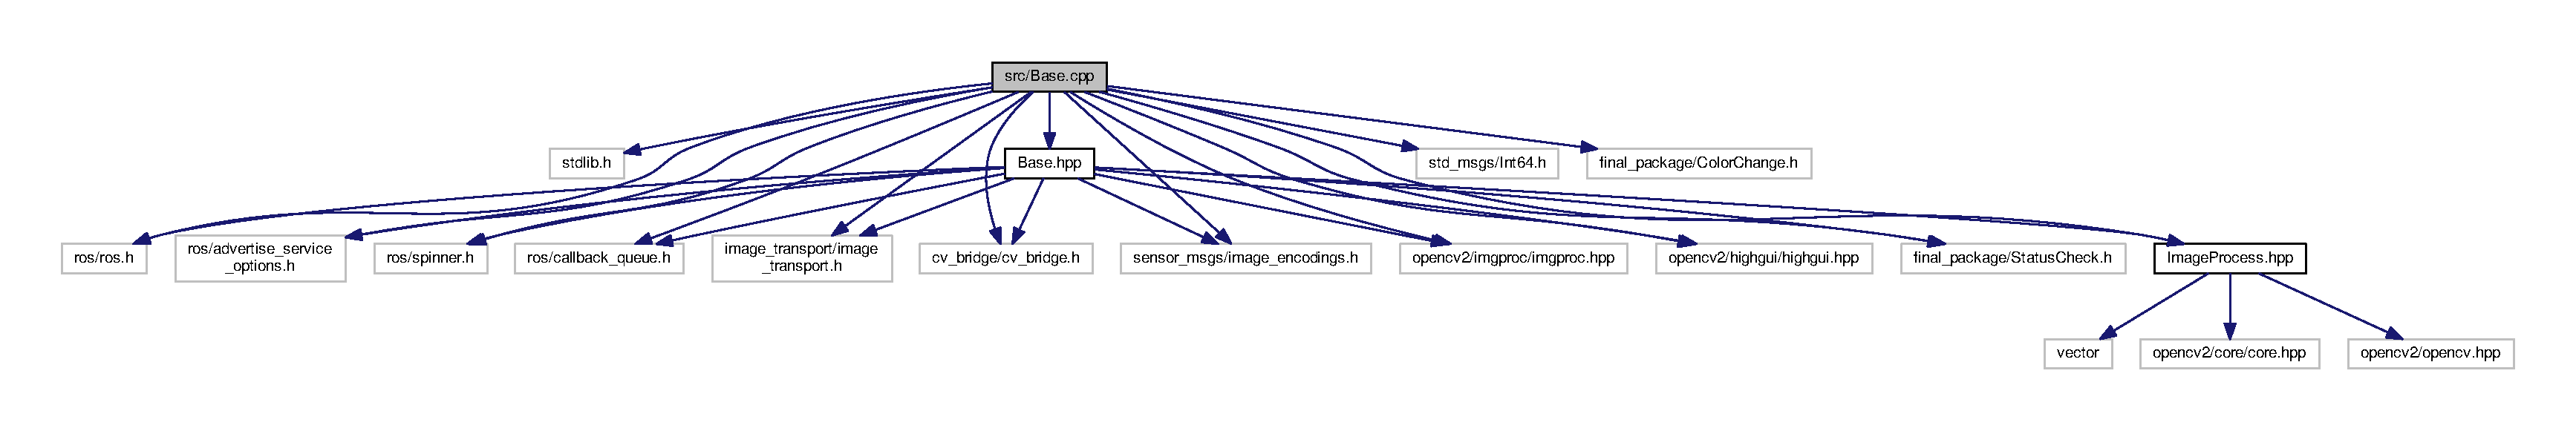
\includegraphics[width=350pt]{Base_8cpp__incl}
\end{center}
\end{figure}


\subsection{Detailed Description}
\hyperlink{classBase}{Base} class implementation source file. 

\begin{DoxyAuthor}{Author}
Yuyu Hsueh  2017, Yuyu Hsueh 
\end{DoxyAuthor}

\hypertarget{base_8cpp}{}\section{src/base.cpp File Reference}
\label{base_8cpp}\index{src/base.\+cpp@{src/base.\+cpp}}


This is a source file for the base node of this project. The base node is responsible of getting and converting the images from the asus-\/xtion\+\_\+pro 3D sensor. Then, it passes these images into an \hyperlink{classImageProcess}{Image\+Process} object, which processes these images and search for the balls\textquotesingle{} centroids. Finally, the displacment between the center of the ball and the center of the image is published to the turtle\+Ctrller node in charge of the turtlebot actuator. In every iteration, the processed image would be displayed in an view window for users to see what the turtlebot sees. There are two services called to make sure all colors of balls are being collected. All the callbacks in this node are running at the rate of 5\+Hz.  


{\ttfamily \#include $<$ros/ros.\+h$>$}\\*
{\ttfamily \#include $<$ros/advertise\+\_\+service\+\_\+options.\+h$>$}\\*
{\ttfamily \#include $<$ros/spinner.\+h$>$}\\*
{\ttfamily \#include $<$ros/callback\+\_\+queue.\+h$>$}\\*
{\ttfamily \#include $<$image\+\_\+transport/image\+\_\+transport.\+h$>$}\\*
{\ttfamily \#include $<$cv\+\_\+bridge/cv\+\_\+bridge.\+h$>$}\\*
{\ttfamily \#include $<$sensor\+\_\+msgs/image\+\_\+encodings.\+h$>$}\\*
{\ttfamily \#include $<$opencv2/imgproc/imgproc.\+hpp$>$}\\*
{\ttfamily \#include $<$opencv2/highgui/highgui.\+hpp$>$}\\*
{\ttfamily \#include \char`\"{}sensor\+\_\+msgs/\+Laser\+Scan.\+h\char`\"{}}\\*
{\ttfamily \#include \char`\"{}final\+\_\+package/\+Color\+Change.\+h\char`\"{}}\\*
{\ttfamily \#include \char`\"{}Base.\+hpp\char`\"{}}\\*
Include dependency graph for base.\+cpp\+:
\nopagebreak
\begin{figure}[H]
\begin{center}
\leavevmode
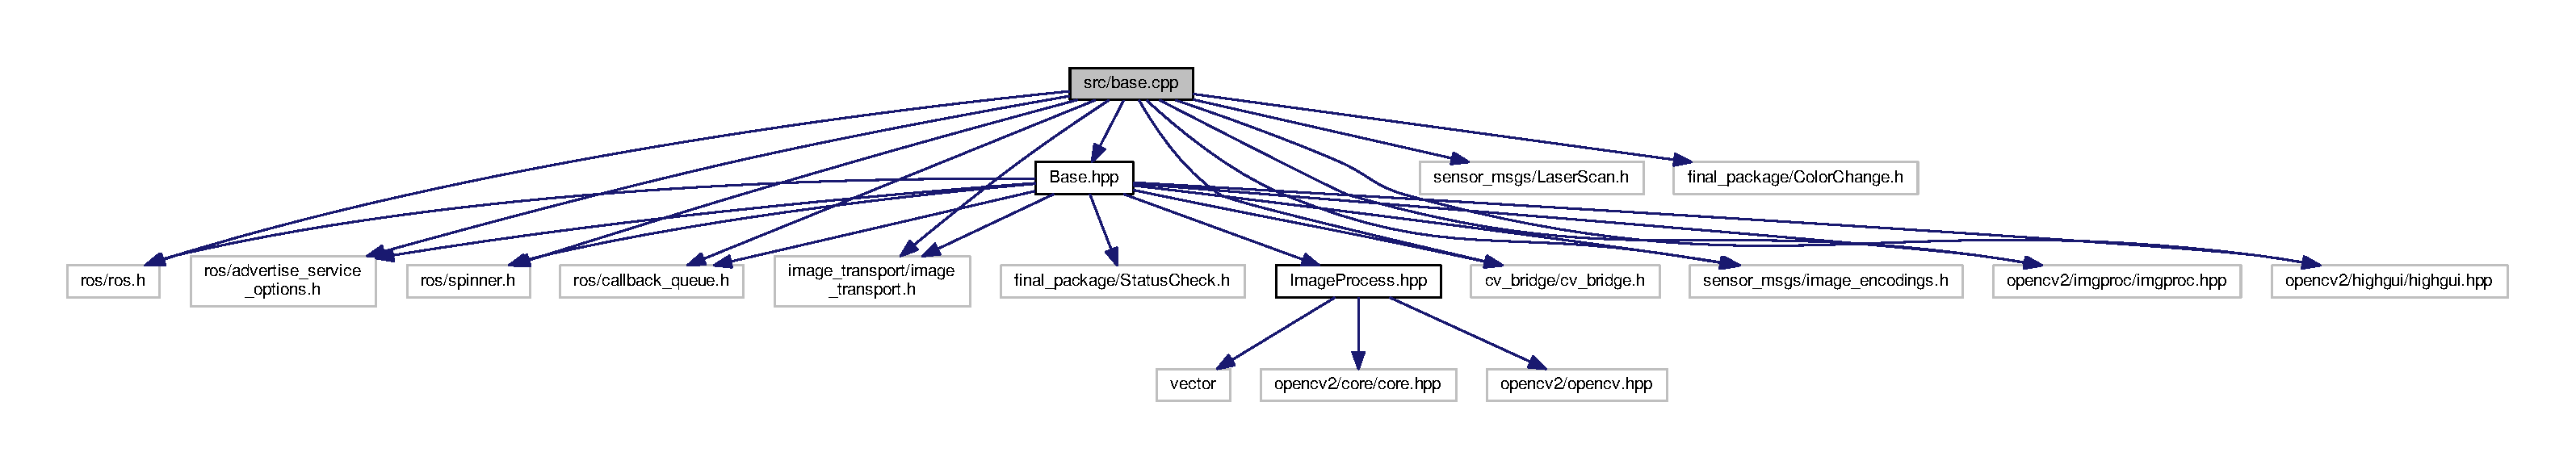
\includegraphics[width=350pt]{base_8cpp__incl}
\end{center}
\end{figure}
\subsection*{Functions}
\begin{DoxyCompactItemize}
\item 
int \hyperlink{base_8cpp_a3c04138a5bfe5d72780bb7e82a18e627}{main} (int argc, char $\ast$$\ast$argv)
\end{DoxyCompactItemize}


\subsection{Detailed Description}
This is a source file for the base node of this project. The base node is responsible of getting and converting the images from the asus-\/xtion\+\_\+pro 3D sensor. Then, it passes these images into an \hyperlink{classImageProcess}{Image\+Process} object, which processes these images and search for the balls\textquotesingle{} centroids. Finally, the displacment between the center of the ball and the center of the image is published to the turtle\+Ctrller node in charge of the turtlebot actuator. In every iteration, the processed image would be displayed in an view window for users to see what the turtlebot sees. There are two services called to make sure all colors of balls are being collected. All the callbacks in this node are running at the rate of 5\+Hz. 

\begin{DoxyAuthor}{Author}
Yuyu Hsueh  2017, Yuyu Hsueh 
\end{DoxyAuthor}


\subsection{Function Documentation}
\index{base.\+cpp@{base.\+cpp}!main@{main}}
\index{main@{main}!base.\+cpp@{base.\+cpp}}
\subsubsection[{\texorpdfstring{main(int argc, char $\ast$$\ast$argv)}{main(int argc, char **argv)}}]{\setlength{\rightskip}{0pt plus 5cm}int main (
\begin{DoxyParamCaption}
\item[{int}]{argc, }
\item[{char $\ast$$\ast$}]{argv}
\end{DoxyParamCaption}
)}\hypertarget{base_8cpp_a3c04138a5bfe5d72780bb7e82a18e627}{}\label{base_8cpp_a3c04138a5bfe5d72780bb7e82a18e627}

\hypertarget{ImageProcess_8cpp}{}\section{src/\+Image\+Process.cpp File Reference}
\label{ImageProcess_8cpp}\index{src/\+Image\+Process.\+cpp@{src/\+Image\+Process.\+cpp}}


This node takes and analyze the range data. Subsequently, pass the the decision made based on the data to the turtle\+Ctrl node which manipulates the turtlebot.  


{\ttfamily \#include $<$ros/ros.\+h$>$}\\*
{\ttfamily \#include $<$opencv2/core/core.\+hpp$>$}\\*
{\ttfamily \#include $<$opencv2/opencv.\+hpp$>$}\\*
{\ttfamily \#include $<$opencv2/imgproc/imgproc.\+hpp$>$}\\*
{\ttfamily \#include $<$opencv2/highgui/highgui.\+hpp$>$}\\*
{\ttfamily \#include \char`\"{}Image\+Process.\+hpp\char`\"{}}\\*
Include dependency graph for Image\+Process.\+cpp\+:
\nopagebreak
\begin{figure}[H]
\begin{center}
\leavevmode
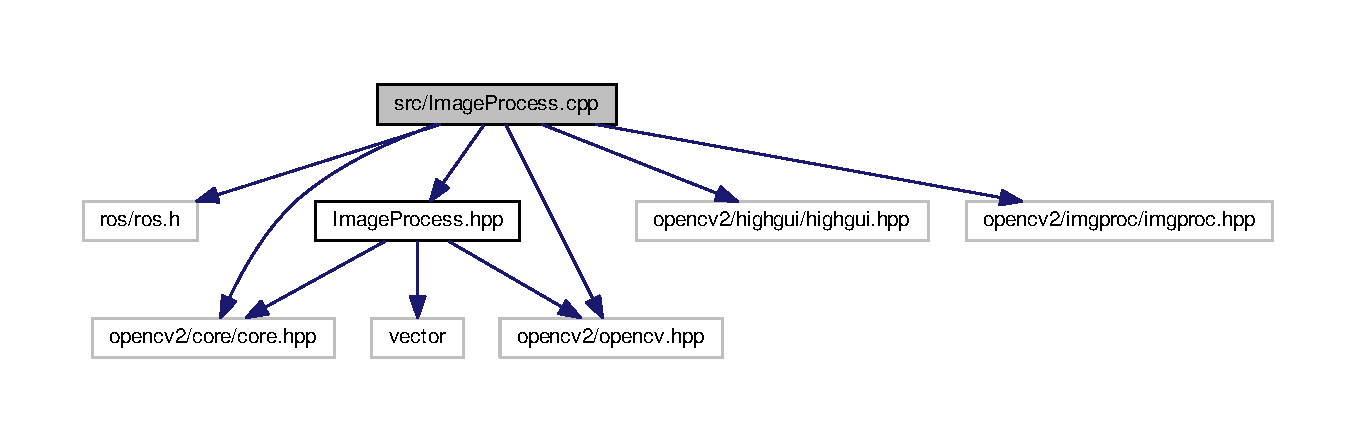
\includegraphics[width=350pt]{ImageProcess_8cpp__incl}
\end{center}
\end{figure}


\subsection{Detailed Description}
This node takes and analyze the range data. Subsequently, pass the the decision made based on the data to the turtle\+Ctrl node which manipulates the turtlebot. 

\begin{DoxyAuthor}{Author}
Yuyu Hsueh  2017, Yuyu Hsueh 
\end{DoxyAuthor}

\hypertarget{TurtleCtrl_8cpp}{}\section{src/\+Turtle\+Ctrl.cpp File Reference}
\label{TurtleCtrl_8cpp}\index{src/\+Turtle\+Ctrl.\+cpp@{src/\+Turtle\+Ctrl.\+cpp}}


This is the implementation file for the \hyperlink{classTurtleCtrl}{Turtle\+Ctrl} class.  


{\ttfamily \#include $<$stdlib.\+h$>$}\\*
{\ttfamily \#include $<$ros/ros.\+h$>$}\\*
{\ttfamily \#include $<$ros/advertise\+\_\+service\+\_\+options.\+h$>$}\\*
{\ttfamily \#include $<$ros/spinner.\+h$>$}\\*
{\ttfamily \#include $<$ros/callback\+\_\+queue.\+h$>$}\\*
{\ttfamily \#include \char`\"{}std\+\_\+msgs/\+Int64.\+h\char`\"{}}\\*
{\ttfamily \#include \char`\"{}std\+\_\+msgs/\+Float32.\+h\char`\"{}}\\*
{\ttfamily \#include \char`\"{}sensor\+\_\+msgs/\+Laser\+Scan.\+h\char`\"{}}\\*
{\ttfamily \#include \char`\"{}geometry\+\_\+msgs/\+Twist.\+h\char`\"{}}\\*
{\ttfamily \#include \char`\"{}Turtle\+Ctrl.\+hpp\char`\"{}}\\*
{\ttfamily \#include \char`\"{}gazebo\+\_\+msgs/\+Delete\+Model.\+h\char`\"{}}\\*
{\ttfamily \#include \char`\"{}final\+\_\+package/\+Color\+Change.\+h\char`\"{}}\\*
{\ttfamily \#include \char`\"{}final\+\_\+package/\+Status\+Check.\+h\char`\"{}}\\*
Include dependency graph for Turtle\+Ctrl.\+cpp\+:
\nopagebreak
\begin{figure}[H]
\begin{center}
\leavevmode
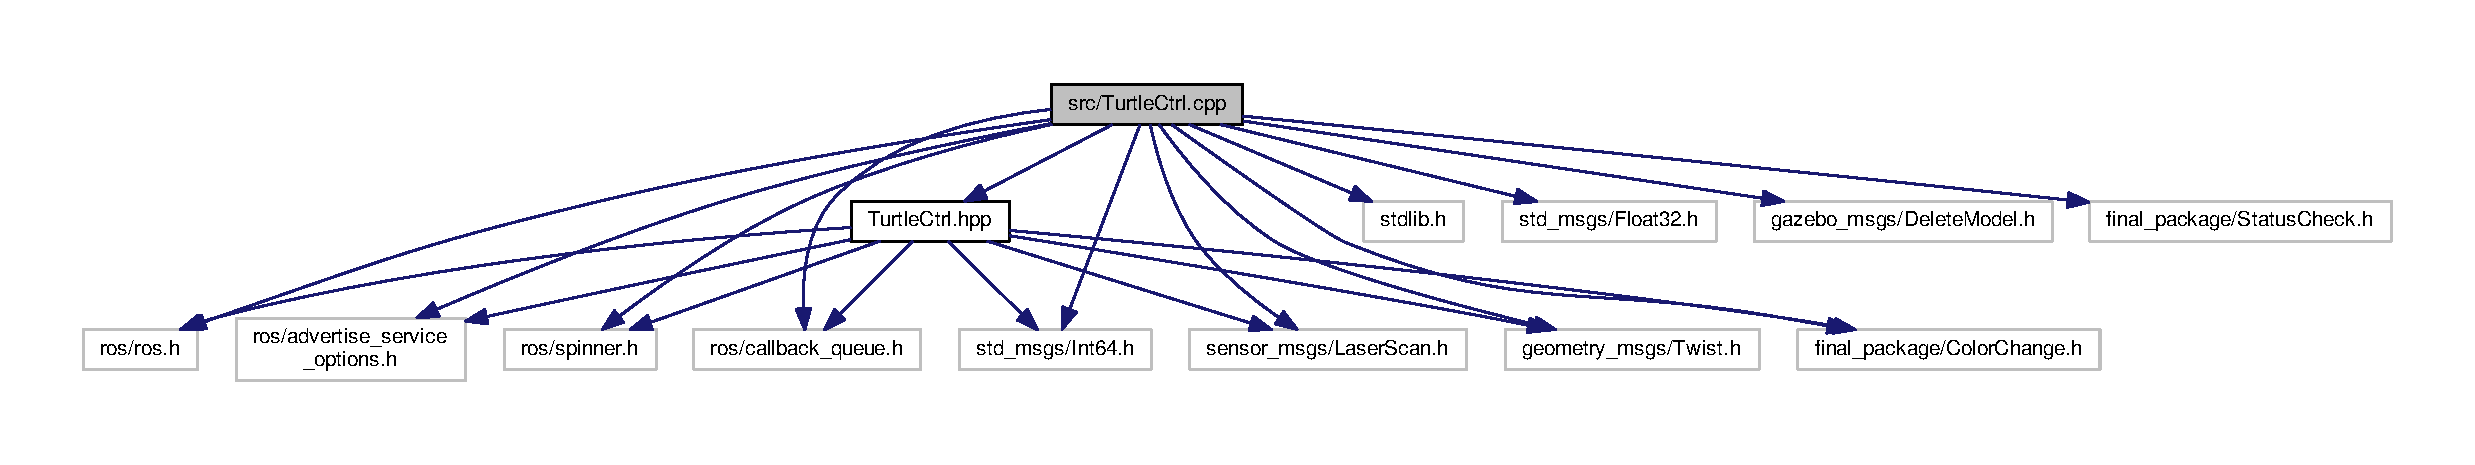
\includegraphics[width=350pt]{TurtleCtrl_8cpp__incl}
\end{center}
\end{figure}


\subsection{Detailed Description}
This is the implementation file for the \hyperlink{classTurtleCtrl}{Turtle\+Ctrl} class. 

\begin{DoxyAuthor}{Author}
Yuyu Hsueh  2017, Yuyu Hsueh 
\end{DoxyAuthor}

\hypertarget{turtleCtrl_8cpp}{}\section{src/turtle\+Ctrl.cpp File Reference}
\label{turtleCtrl_8cpp}\index{src/turtle\+Ctrl.\+cpp@{src/turtle\+Ctrl.\+cpp}}


This is the source code for the turtle\+Ctrller node, which has a simple PD controller that takes the displacement value as input. The output is published to the turtlebot actuator in terms of linear and angular velocities.  


{\ttfamily \#include \char`\"{}ros/ros.\+h\char`\"{}}\\*
{\ttfamily \#include $<$ros/spinner.\+h$>$}\\*
{\ttfamily \#include $<$ros/callback\+\_\+queue.\+h$>$}\\*
{\ttfamily \#include \char`\"{}Turtle\+Ctrl.\+hpp\char`\"{}}\\*
Include dependency graph for turtle\+Ctrl.\+cpp\+:\nopagebreak
\begin{figure}[H]
\begin{center}
\leavevmode
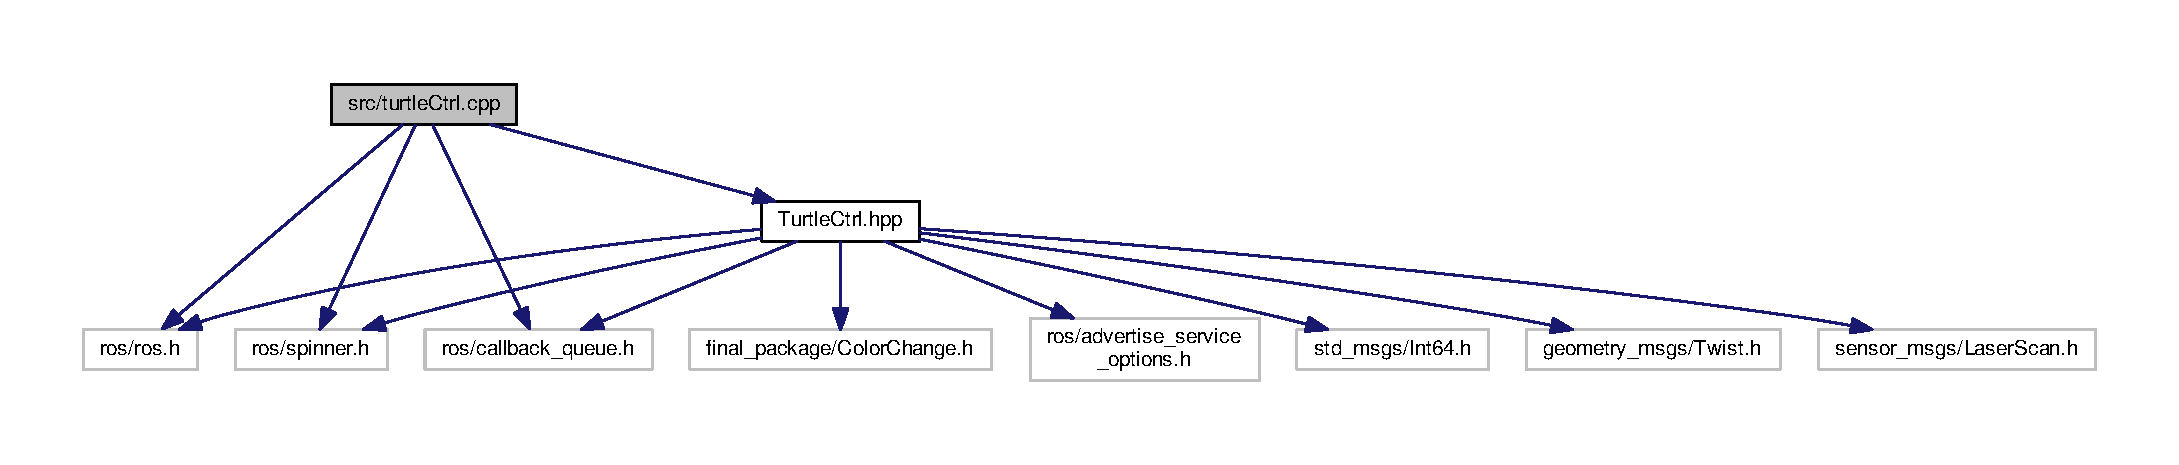
\includegraphics[width=350pt]{turtleCtrl_8cpp__incl}
\end{center}
\end{figure}
\subsection*{Functions}
\begin{DoxyCompactItemize}
\item 
int \hyperlink{turtleCtrl_8cpp_a3c04138a5bfe5d72780bb7e82a18e627}{main} (int argc, char $\ast$$\ast$argv)
\end{DoxyCompactItemize}


\subsection{Detailed Description}
This is the source code for the turtle\+Ctrller node, which has a simple PD controller that takes the displacement value as input. The output is published to the turtlebot actuator in terms of linear and angular velocities. 

\begin{DoxyAuthor}{Author}
Yuyu Hsueh  2017, Yuyu Hsueh 
\end{DoxyAuthor}


\subsection{Function Documentation}
\index{turtle\+Ctrl.\+cpp@{turtle\+Ctrl.\+cpp}!main@{main}}
\index{main@{main}!turtle\+Ctrl.\+cpp@{turtle\+Ctrl.\+cpp}}
\subsubsection[{\texorpdfstring{main(int argc, char $\ast$$\ast$argv)}{main(int argc, char **argv)}}]{\setlength{\rightskip}{0pt plus 5cm}int main (
\begin{DoxyParamCaption}
\item[{int}]{argc, }
\item[{char $\ast$$\ast$}]{argv}
\end{DoxyParamCaption}
)}\hypertarget{turtleCtrl_8cpp_a3c04138a5bfe5d72780bb7e82a18e627}{}\label{turtleCtrl_8cpp_a3c04138a5bfe5d72780bb7e82a18e627}

\hypertarget{base__test_8cpp}{}\section{test/base\+\_\+test.cpp File Reference}
\label{base__test_8cpp}\index{test/base\+\_\+test.\+cpp@{test/base\+\_\+test.\+cpp}}
{\ttfamily \#include $<$ros/ros.\+h$>$}\\*
{\ttfamily \#include $<$gtest/gtest.\+h$>$}\\*
{\ttfamily \#include \char`\"{}sensor\+\_\+msgs/\+Laser\+Scan.\+h\char`\"{}}\\*
{\ttfamily \#include \char`\"{}std\+\_\+msgs/\+Float32.\+h\char`\"{}}\\*
{\ttfamily \#include $<$opencv2/highgui/highgui.\+hpp$>$}\\*
{\ttfamily \#include $<$cv\+\_\+bridge/cv\+\_\+bridge.\+h$>$}\\*
{\ttfamily \#include $<$opencv2/core/core.\+hpp$>$}\\*
{\ttfamily \#include $<$opencv2/opencv.\+hpp$>$}\\*
{\ttfamily \#include $<$iostream$>$}\\*
Include dependency graph for base\+\_\+test.\+cpp\+:\nopagebreak
\begin{figure}[H]
\begin{center}
\leavevmode
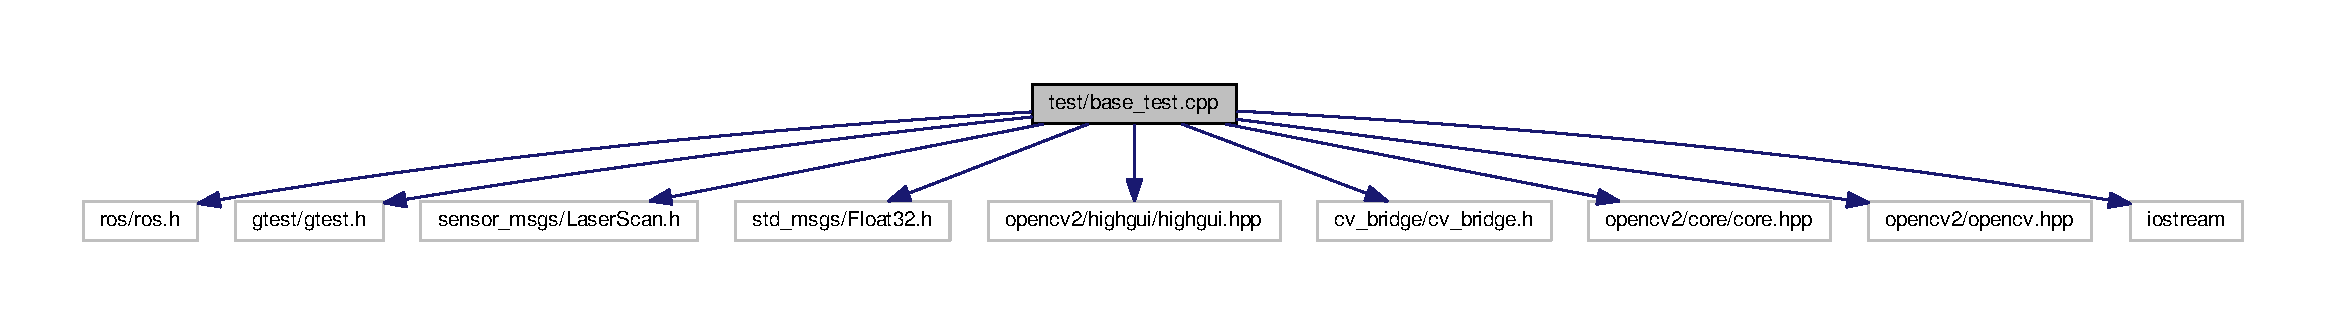
\includegraphics[width=350pt]{base__test_8cpp__incl}
\end{center}
\end{figure}
\subsection*{Functions}
\begin{DoxyCompactItemize}
\item 
void \hyperlink{base__test_8cpp_adeb905f276d222fa4eb1e4954e07ae03}{distance\+Callback} (const std\+\_\+msgs\+::\+Float32\+::\+Const\+Ptr \&msg)
\item 
\hyperlink{base__test_8cpp_ac4f819542112ad90f9f02dba76320e63}{T\+E\+ST} (integration\+Test, range\+\_\+call\+\_\+back)
\item 
int \hyperlink{base__test_8cpp_a3c04138a5bfe5d72780bb7e82a18e627}{main} (int argc, char $\ast$$\ast$argv)
\end{DoxyCompactItemize}
\subsection*{Variables}
\begin{DoxyCompactItemize}
\item 
std\+::shared\+\_\+ptr$<$ ros\+::\+Node\+Handle $>$ \hyperlink{base__test_8cpp_a7d6d3de9ddf4963eb3ea112920944a87}{nh}
\item 
float \hyperlink{base__test_8cpp_aa464047f090200f942a1e47c29fff783}{min\+\_\+dist}
\end{DoxyCompactItemize}


\subsection{Function Documentation}
\index{base\+\_\+test.\+cpp@{base\+\_\+test.\+cpp}!distance\+Callback@{distance\+Callback}}
\index{distance\+Callback@{distance\+Callback}!base\+\_\+test.\+cpp@{base\+\_\+test.\+cpp}}
\subsubsection[{\texorpdfstring{distance\+Callback(const std\+\_\+msgs\+::\+Float32\+::\+Const\+Ptr \&msg)}{distanceCallback(const std_msgs::Float32::ConstPtr &msg)}}]{\setlength{\rightskip}{0pt plus 5cm}void distance\+Callback (
\begin{DoxyParamCaption}
\item[{const std\+\_\+msgs\+::\+Float32\+::\+Const\+Ptr \&}]{msg}
\end{DoxyParamCaption}
)}\hypertarget{base__test_8cpp_adeb905f276d222fa4eb1e4954e07ae03}{}\label{base__test_8cpp_adeb905f276d222fa4eb1e4954e07ae03}
Testing case confirming that the messages passed between service and client are same. \index{base\+\_\+test.\+cpp@{base\+\_\+test.\+cpp}!main@{main}}
\index{main@{main}!base\+\_\+test.\+cpp@{base\+\_\+test.\+cpp}}
\subsubsection[{\texorpdfstring{main(int argc, char $\ast$$\ast$argv)}{main(int argc, char **argv)}}]{\setlength{\rightskip}{0pt plus 5cm}int main (
\begin{DoxyParamCaption}
\item[{int}]{argc, }
\item[{char $\ast$$\ast$}]{argv}
\end{DoxyParamCaption}
)}\hypertarget{base__test_8cpp_a3c04138a5bfe5d72780bb7e82a18e627}{}\label{base__test_8cpp_a3c04138a5bfe5d72780bb7e82a18e627}
\index{base\+\_\+test.\+cpp@{base\+\_\+test.\+cpp}!T\+E\+ST@{T\+E\+ST}}
\index{T\+E\+ST@{T\+E\+ST}!base\+\_\+test.\+cpp@{base\+\_\+test.\+cpp}}
\subsubsection[{\texorpdfstring{T\+E\+S\+T(integration\+Test, range\+\_\+call\+\_\+back)}{TEST(integrationTest, range_call_back)}}]{\setlength{\rightskip}{0pt plus 5cm}T\+E\+ST (
\begin{DoxyParamCaption}
\item[{integration\+Test}]{, }
\item[{range\+\_\+call\+\_\+back}]{}
\end{DoxyParamCaption}
)}\hypertarget{base__test_8cpp_ac4f819542112ad90f9f02dba76320e63}{}\label{base__test_8cpp_ac4f819542112ad90f9f02dba76320e63}
Sending fake laserscan measurment and subscribe to the base node and see if the result is expected. 

\subsection{Variable Documentation}
\index{base\+\_\+test.\+cpp@{base\+\_\+test.\+cpp}!min\+\_\+dist@{min\+\_\+dist}}
\index{min\+\_\+dist@{min\+\_\+dist}!base\+\_\+test.\+cpp@{base\+\_\+test.\+cpp}}
\subsubsection[{\texorpdfstring{min\+\_\+dist}{min_dist}}]{\setlength{\rightskip}{0pt plus 5cm}float min\+\_\+dist}\hypertarget{base__test_8cpp_aa464047f090200f942a1e47c29fff783}{}\label{base__test_8cpp_aa464047f090200f942a1e47c29fff783}
\index{base\+\_\+test.\+cpp@{base\+\_\+test.\+cpp}!nh@{nh}}
\index{nh@{nh}!base\+\_\+test.\+cpp@{base\+\_\+test.\+cpp}}
\subsubsection[{\texorpdfstring{nh}{nh}}]{\setlength{\rightskip}{0pt plus 5cm}std\+::shared\+\_\+ptr$<$ros\+::\+Node\+Handle$>$ nh}\hypertarget{base__test_8cpp_a7d6d3de9ddf4963eb3ea112920944a87}{}\label{base__test_8cpp_a7d6d3de9ddf4963eb3ea112920944a87}

%--- End generated contents ---

% Index
\backmatter
\newpage
\phantomsection
\clearemptydoublepage
\addcontentsline{toc}{chapter}{Index}
\printindex

\end{document}
